% This is samplepaper.tex, a sample chapter demonstrating the
% LLNCS macro package for Springer Computer Science proceedings;
% Version 2.20 of 2017/10/04
%
\documentclass[runningheads]{llncs}
%
\usepackage{minted}
\usepackage{pgf}
\usepackage{import}
\usepackage{layouts}
\usepackage{graphicx}
\usepackage{tikz}
\usetikzlibrary{shapes.geometric, arrows}
\usepackage{amsmath}
\usepackage{adjustbox}
\usepackage{placeins}
\usepackage{float}
\usepackage{xspace}
\usepackage{array}
\usepackage{tabularx,booktabs}\usepackage[hidelinks]{hyperref}
\usepackage{cleveref}
\usepackage{afterpage}
\usepackage{svg}
\usepackage{xcolor}
\usepackage{appendix}
\newcolumntype{Y}{>{\centering\arraybackslash}X}


% Used for displaying a sample figure. If possible, figure files should
% be included in EPS format.
%
% If you use the hyperref package, please uncomment the following line
% to display URLs in blue roman font according to Springer's eBook style:
% \renewcommand\UrlFont{\color{blue}\rmfamily}

\renewcommand\#{\protect\scalebox{0.8}{\protect\raisebox{0.4ex}{\char"0023}}}
\definecolor{darkgrey}{RGB}{100,100,100} 
\newcommand{\sort}{SAMtools \texttt{sort}\xspace}
\newcommand{\points}{Data points: Median, Error bars: Fastest and slowest of 3 runs. }
\newcommand{\parents}{Numbers in parentheses indicate the compression level. }
\newcommand{\threads}{One thread is single threaded computation, for a higher thread count, \sort uses the threads in addition to the main thread. }
\interfootnotelinepenalty=100000


\begin{document}


%
\title{Faster Sorting of Aligned DNA-Read Files}
%
%\titlerunning{Abbreviated paper title}
% If the paper title is too long for the running head, you can set
% an abbreviated paper title here
%
\author{Dominik Siebelt}
% Second Author\inst{2,3}\orcidID{1111-2222-3333-4444} \and
% Third Author\inst{3}\orcidID{2222--3333-4444-5555}}
%
\authorrunning{D. Siebelt}
% First names are abbreviated in the running head.
% If there are more than two authors, 'et al.' is used.
%
\institute{Karlsruhe Institute of Technology}
% Springer Heidelberg, Tiergartenstr. 17, 69121 Heidelberg, Germany
% \email{lncs@springer.com}\\
% \url{http://www.springer.com/gp/computer-science/lncs} \and
% ABC Institute, Rupert-Karls-University Heidelberg, Heidelberg, Germany\\
% \email{\{abc,lncs\}@uni-heidelberg.de}}
%
\maketitle              % typeset the header of the contribution
%
% \begin{abstract}
% The abstract should briefly summarize the contents of the paper in
% 15--250 words.

% \keywords{First keyword  \and Second keyword \and Another keyword.}
% \end{abstract}
%
\setcounter{tocdepth}{2}
\tableofcontents
\newpage
%
\section{Introduction}
Analysis of aligned DNA-Read data is a crucial part of modern bioinformatics with applications for scientific and medical purposes. DNA-Reads are small sequences of DNA sequences coming off a DNA sequencing machine. They are then aligned to a reference sequence to find variants, disease causing mutations and understand evolutionary relationships between species. In order to analyze specific parts of a genome, such as a chromosome and to locate mutations or variations, DNA-Reads are sorted. This also improves the performance of many other downstream analysis tasks, for example finding and removing duplicate reads. \\

To address the vast amounts of data generated by modern DNA sequencing machines, highly efficient tools and data formats are needed. Developed during the 1000 Genome Project~\cite{the_1000_genomes_project_consortium_1000_2012}, the SAM and BAM formats for storing alignment information to DNA sequences, have found widespread use. Developed alongside these formats, SAMtools became a standard tool for manipulating SAM and BAM files. Next to a collection of many different commands for filtering DNA-Reads, merging of aligned DNA-Read files and many more, SAMtools offers with \sort a tool to alternate the order of the DNA sequences stored in DNA-Read files such as SAM and BAM files. \\

This thesis is about speeding up \sort at sorting DNA-Reads in BAM files with the goal of reducing computation costs and time. BAM is a file format capable of alignment information to DNA sequences in a binary and compressed way. Since DNA data typically occupies substantial storage space, compression is build into the BAM file format in order to reduce storage space and costs, as well as to enable faster transfer over the network.\\

\sort can arrange DNA-Read files in various orders. The default order involves sorting by the reference sequence to which a DNA read is mapped, followed by the position of the mapping on this reference sequence. This enables fast random access to specific regions of interest via index files. \\

Index files are used in the handling of BAM files to facilitate random access despite compression. BAM files are compressed with a special compression method allowing to access the content of the file in blocks without the necessity of decompressing all preceding blocks of the file. The compression format internally uses the compression library zlib for GZIP for compression, which is one of the most popular compression methods. With zlib being open source and used extensively in various applications such as web servers and communication, other libraries have been implemented, offering zlib compatible compression with higher throughput and higher compression efficiency. \\

In this thesis, I present three approaches to speed up the sorting of DNA-Reads stored in BAM files utilizing \sort. \\

\sort performs an external memory sort. If not enough memory is available to \sort, it writes temporary files. If it writes a larger amount of them, it merges them, which is computational intensive. In this thesis, I analyze the impacts of \sort writing and merging temporary files. I propose parameter settings and changes in \sort's internal limitation setting, reducing the amount of merges and thus lowering the computation time of \sort. \\

\sort dedicates a significant amount of its runtime to compressing temporary and output files. To maintain the advantages of compression but reduce its impact on \sort's total runtime, I examine various zlib-compatible compression libraries and the effects of different compression levels. \\

At last, I assess the impacts of IO operations and limitations of IO devices and propose recommendations to minimize or eliminate them.



\subsection{SAMtools}
SAMtools~\cite{12ySamtools} is a collection of tools to work on alignment data, such as aligned DNA-Reads. It relies on the co-developed HTSlib~\cite{bonfield_htslib_2021} for reading and writing information files, e.g. BAM files. SAMtools offers functionality for different operations on alignment data, such as format conversion, statistics, variant calling and many more, including the sorting, which is the focus here. \\

\subsection{Aligned DNA-Reads}
DNA-Reads are sequences of bases coming from a sequencing machine. They can consist of multiple contiguous sequences. Aligned DNA-Reads are DNA-Reads aligned to a reference sequence. The alignment may include insertions, deletions, mismatches, and skipped parts of the reference sequence. Additionally, clipping removes low-quality portions of the sequenced fragment to improve the alignment of the remaining high-quality sequence with the reference. Also, changes in directions on the reference are possible.

\subsection{SAM and BAM files}
A Sequence Alignment Map (SAM) as specified by Li et al.~\cite{samformat} is used to store the alignment of sequences against reference sequences. It consists of a header section and an alignment section. The header section contains meta information such as the format version or the sorting of the content and a dictionary of the reference sequences, whereas the alignment section contains aligned segments with alignment information and meta information such as the read quality. A segment is a continuous sequence or subsequence of a raw DNA-Read. Aligned DNA-Reads are eventually put into multiple records with different segments in the alignment section, as single BAM records can not store changes in directions of the alignment on the reference sequence.\\

The alignment information primarily includes the ID of the reference sequence to which the alignment is mapped, the position in the reference sequence where the alignment starts, and a CIGAR string detailing the alignment at this position. The CIGAR String consists of a list of symbols representing sequential matches, mismatches, insertions, and deletions. Therefore, it represents the alignment of the corresponding segment and its reference sequence. \\

A BAM file is the binary representation of a SAM file. The main differences are the usage of a 4-bit encoding for the sequences, a 3-bit encoding for CIGAR Symbols and a 0-based instead of 1-based coordinate system for the position. Furthermore, a BAM file is per default \textit{BGZF} compressed.

\subsection{BGZF Compression} \label{bgzf}
BGZF, short for Blocked GNU Zip Format, is a lossless compression method proposed at the same time as the BAM format. Widely used compression methods like GZIP compress a file from the beginning to the end in one piece. This has the advantage of allowing matching segments of the file to be located over a greater range. Thus, the compression method is able to reduce the file size more effectively, as repeated sequences can be identified throughout the entire file. However, to decompress such a compressed file, it also needs to be read from the beginning and, depending on the compression method, decompressed at least until the point of interest. \\

Since alignment data can produce very large files but not all of their regions are needed for every use case, it is beneficial to enable some form of random access. To archive this, BGZF utilizes GZIP~\cite{gzip} to compress large files into blocks of less than 64\,KB size (compressed and uncompressed). GZIP uses the DEFLATE algorithm~\cite{deflate} by Phil Katz to compress these individual blocks, which it then subsequently concatenates. Thus, fast random access using index files is possible. In an index file, the position of a piece of information is stored in a 64-bit integer. It consists of a 48-bit unsigned integer \textit{coffset} indicating the number of the compressed block and a 16-bit unsigned integer \textit{uoffset} describing the position in the uncompressed block. \\

Also, the BGZF format provides compatibility with GZIP. Any file compressed utilizing BGZF can be decompressed by any standard GZIP decompression implementation, as GZIP allows this combination of multiple compressed files to one file. Given that Gzip is highly prevalent as a compression technique, there are numerous compatible compression and decompression libraries for all platforms. Thus, employing the open-source GZIP internally simplifies the development of other legacy tools working with BGZF-compatible compression.  \\

Like GZIP, BGZF supports compression levels ranging from 1 (fastest but worst) to 9 (slowest but best) mirroring the compression levels used for the underlying GZIP compression. The compression levels affect the size of the compressed files, as shown in Figure~\ref{fig:compSizes}.
\begin{figure}[t]
        \import{figures/}{compSizes.pgf}
    \caption{Comparison of the size of BGZF compressed files on all compression levels, exemplified using a 10.4\,GiB unsorted BAM file. \\
    Although no compression yields a file four times as large, the distinctions between compression levels are less significant.}
    \label{fig:compSizes}
\end{figure}
The speed of the compression depends mainly on the compression level, the GZIP-implementation and the number of used threads (see Figure \ref{fig:compSpeed}).  
\begin{figure}
        \import{figures/}{compSpeed.pgf}
    \caption{Comparison of the output rate of HTSlib's \texttt{bgzip} which uses BGZF to compress A 10.4GiB unsorted BAM file. For reference, compression level 0 is plotted in the smaller inset plot. \\
    While no compression significantly outpaces every compression level, the throughput increments between the compression levels are consistent.}
    \label{fig:compSpeed}
\end{figure}
To measure the compression speed, I measure the speed of HTSlib's \texttt{bgzip}. This is a tool to compress arbitrary files using BGZF. \sort uses the same methods as \texttt{bgzip} of HTSlib, the library utilized by SAMtools for compression and file operations. This still holds for compression level 0. For this compression level, \texttt{bgzip} as well as \sort do not compress, but directly written the output. Therefore, the compression speed of \texttt{bgzip} is relevant for sorting because it sets a lower boundary on writing the output of \sort, considering that \sort also needs to compress its output.

\section{Prerequisites}

\subsection{SAMtools}
SAMtools~\cite{12ySamtools} is a collection of tools to work on alignment data, such as aligned DNA-Reads. It relies on the co-developed HTSlib~\cite{bonfield_htslib_2021} for reading and writing information files, namely SAM, BAM, and CRAM files. With \sort, SAMtools offers functionality for sorting of aligned DNA-Read files, which is the focus here. In addition, SAMtools offers functionality for different operations on alignment data, such as format conversion, statistics, variant calling and many more.

\subsection{Aligned DNA-Reads}
DNA-Reads are short (typically 250–800 nucleotides long~\cite{hu_next-generation_2021}) sequences of nucleotides, the fundamental building blocks of DNA. These nucleotides are denoted by their bases, adenine (\texttt{A}), guanine (\texttt{G}), cytosine (\texttt{C}), and thymine (\texttt{T}). A DNA-Read can consist of multiple contiguous sequences. 

Aligned DNA-Reads are DNA-Reads aligned to a reference sequence, which serves as
a standard DNA or RNA sequence for comparison within a species. The alignment may include insertions, deletions, mismatches, and skipped parts of the reference sequence. Additionally, a step called \textit{clipping} excludes parts of the sequenced fragment with low read qualities from the alignment to improve the alignment of the remaining high-quality sequence with the reference sequence. Also, changes in the direction of the alignment on the reference are possible. In alignment files, changes in direction of the alignment lead to splitting up the DNA-Read into multiple sequences, one for each contiguous part of the DNA-Read aligned in the same direction.

\subsection{SAM and BAM files}
A SAM (Sequence Alignment Map) file as specified by Li et al.~\cite{samformat} is used to store the alignment of sequences against reference sequences. It consists of a header section and an alignment section. The header section contains meta information such as the format version or the sorting of the content and a dictionary of the reference sequences, whereas the alignment section contains aligned segments with alignment information and meta information such as the read quality. A segment is a continuous sequence or subsequence of a raw DNA-Read. Aligned DNA-Reads are eventually put into multiple records with different segments in the alignment section, as single BAM records can not store changes in directions of the alignment on the reference sequence.

The alignment information primarily includes the ID of the reference sequence to which the alignment is mapped, the position in the reference sequence where the alignment starts, and detail on the alignment of this position (match, mismatch, insertion, or deletion). 

A BAM (Binary Alignment Map) file is the binary representation of a SAM file. Compared to the SAM format, this format utilizes a 4-bit encoding for DNA sequences, a 3-bit encoding for CIGAR symbols, and adopts a 0-based coordinate system for positions. Furthermore, a BAM file is per default \textit{BGZF} compressed.

\subsection{The DEFLATE format and algorithm}
The DEFLATE format~\cite{deflate} is a format specifying data compressed with a combination of an LZ77 algorithm~\cite{ziv_universal_1977} and Huffman Coding~\cite{huffman_method_1952}. Compressed data is structured as a sequence of consecutive blocks. These blocks contain strings and references to previous strings (matches). The references to previous strings contain the distance to and the length of the matching part. The bytes of the strings which are no matches to previous strings and the pointers, which consist of distances and lengths, are compressed using Huffman coding. The trees representing the Huffman codes are Huffman coded as well. 
The DEFLATE algorithm is an algorithm capable of producing an output stream in the DEFLATE format given an input data stream.

\subsection{GZIP and zlib}
GZIP~\cite{gzip} is a container format for data compressed in the DEFLATE format. A GZIP file consists of a series of \textit{members} which consist of a header, a series of compressed blocks, and a footer. The header contains meta information on the compressed files (e.g., the file name and the modification time) and can also contain extra fields which in the BGZF file format are used to identify a member as part of a BGZF file and store the length of the compressed member. The compressed blocks contain the compressed data and the footer contains a checksum and the size of the uncompressed content of the blocks modulo $2^{32}$. 

The c library zlib is an implementation of the DEFLATE algorithm. It can produce output in GZIP, ZLIB, or raw DEFLATE format. The ZLIB format is a wrapper for DEFLATE similar to the GZIP format but with less header information and another checksum algorithm (Adler32 instead of crc32).


\subsection{BGZF Compression} \label{bgzf}
The Blocked GNU Zip Format (BGZF) is a lossless compression method proposed together with the BAM format. Widely used compression methods like GZIP compress a file from the beginning to the end in one piece. This has the advantage of allowing matching segments of the file to be located over a greater range. Thus, the compression method is able to reduce the file size more effectively, as repeated sequences can be identified throughout the entire file. However, to decompress such a compressed file, it also needs to be read from the beginning and, depending on the compression method, decompressed at least until the point of interest. 

Given that not all regions of large alignment data files are relevant for every analysis, random access is required for efficient analysis of specific data subsets. To achieve this, BGZF utilizes GZIP~\cite{gzip} to compress large files into blocks of less than 64\,KB size (compressed and uncompressed). GZIP uses the DEFLATE algorithm~\cite{deflate} to compress these individual blocks, which it then subsequently concatenates. Thus, fast random access using index files is possible. In an index file, the position of a piece of information is stored as a 64\,bit integer. This index is divided into a 48\,bit block index and a 16\,bit offset in the respective block.

The BGZF format leverages compatibility with GZIP, enabling any standard GZIP decompression tool to handle BGZF-compressed files. This compatibility stems from BGZF exploiting GZIP's ability to combine multiple compressed blocks into a single file. Given that Gzip is highly prevalent as a compression technique, there are numerous compatible compression and decompression libraries for all platforms. Thus, employing the open-source GZIP internally simplifies the development of other legacy tools working with BGZF-compatible compression.  

Like GZIP, BGZF supports compression levels ranging from 1 (fastest but largest file size) to 9 (slowest but smallest file size) analogously to the compression levels used for the underlying GZIP compression. We show detail on the resulting files sizes and throughput differences between the compression levels in \Cref{clevels}.


\FloatBarrier
\newpage % Zwischen Chapter kann man sich ein Seitenumbruch gönnen.
\section{Related Work}

\subsection{Sorting Tools}
SAMtools is the most commonly used tool for manipulating SAM and BAM files, which store information on aligned DNA-Reads. With over 5.1~Million downloads (05.2014), it is the most downloaded package from the Bioconda~\cite{the_bioconda_team_bioconda_2018} channel, which is a common source for bioinformatic tools in the package and dependency manager Conda. However, there are some alternatives for sorting aligned DNA-Read files, such as sambamba~\cite{tarasov_sambamba_2015}, Picard~\cite{Picard2019toolkit} and NovoSort~\cite{noauthor_novosort_nodate}. Picard, written in Java, provides a simpler interface for sorting SAM and BAM files, but its functions are limited compared to sort, and it does not prioritize efficiency. NovoSort is a commercial program and, therefore, I could not test it. Sambamba, written in the D programming language~\cite{alexandrescu_d_2010}, aims to provide a subset of SAMtools functionality, including sort, but with greater efficiency through higher parallelization. Sambamba reached this goal during its implementation in 2012 as SAMtools. However, with SAMtools introducing parallelism in version 1.4 in 2017, this advantage diminished.\\

\subsection{Compression Methods and Ouput Files}
Compression using BGZF, which is part of the specification of BAM files utilizes GZIP. As a general purpose compression method, GZIP is not specialized in compression DNA data. Hence, a variety of compression algorithms have been developed specifically for DNA data~\cite{hosseini_survey_2016}. These algorithms aim to minimize the resulting file size, compression speed, memory usage during compression or decompression, or decompression speed, but typically focus primarily on minimizing the resulting file size. Compression algorithms are divided in \textit{reference-based} and \textit{reference-free} methods. \\

Reference-based algorithms utilize the reference sequence a DNA-Read is aligned too. By only storing differences between each DNA-Read sequence and the reference sequence, they archive better compression. NGC~\cite{popitsch_ngc_2013} is an example for this, which also splits the kind of data, namely the sequences, sequence names, read qualities and so on in different blocks and compresses them seperately. Other algorithms like Goby~\cite{campagne_compression_2013}, DeeZ~\cite{hach_deez_2014}, and CRAM~\cite{fritz_efficient_2011} are also reference-based, but keep the advantage of enabling random access through index files. CRAM (Compressed Reference-oriented Alignment Map) is also built into HTSlib, the library SAMtools utilizes for file operations, and the user can choose to use it as output for \sort. NGC, Goby and CRAM also offer lossy compression. Lossy compression mainly removes meta information or applies lossy compression to the read qualities of DNA-reads, as their exact value is not always needed, it does not depend on the alignment and is thus hard to compress lossless. Although reference compression methods for SAM files are still actively developed~\cite{banerjee_abridge_2022}, they lack interoperability, as the compression methods are not widely used. An exception to this is CRAM, which is supported by HTSlib. Although CRAM files offer several advantages over BAM files, BAM files remain more popular due to their wider support among software tools.\\

Reference-free compression methods like BGZF, which is used in BAM files per specification, offer the advantage of not needing the reference sequence for compression and decompression. In addition, reference-based compression methods often require the DNA-Reads to be sorted. As this is not necessary for reference-free compression methods, they are more flexible. However, the only commonly used reference-free compression method is the BAM format, which uses binary encoding for the bases a DNA sequence consists of and BGZF compression. \\

In summary, the BAM file format employing BGZF compression, which internally utilizes GZIP, is the most commonly used format for storing aligned DNA-Reads. Given its widespread use, optimizing the speed of generating BAM files using \sort is essential. However, the increasing adoption of the CRAM format might lessen the future significance of BAM file generation.


\newpage
\section{Analysis (Version 1.19.2)}

\subsection{Algorithm}
\subsubsection{Prerequisites}
The process of sorting alternates, depending on some internal Constants and command-line-arguments: \\
We only focus on sorting by the order of the reference, then position and then the REVERSE flag which indicates, if the sequence is aligned forward or backward to the reference. This order is the one used by SAMtools per default, although other sorting criteria e.g. tags or the read name are possible.\\
The maximum amount of memory used to sorting is calculated by the amount of memory the user specifies via the \texttt{-m} option multiplied by the (via \texttt{-@} option) assigned number of threads. Here, we refer to the total amount as \texttt{max\_mem}. \\
The in- and output formats are per default inferred from the file names. \\
SAMtools \texttt{sort} passes its output to standard output if no output file is specified. In this case, the output format is set to BAM.
The maximum number of temporary files is hard-coded as 64 in a constant named \texttt{MAX\_TMP\_FILES}. \\
The gzip compression level for temporary files is set to 1, while the compression level of the result file can be changed via the \texttt{-l} parameter. It defaults to the default compression level used by the library that implements the compression, usually 6, but can be set to a number between 0 (no compression) and 9 (highest and slowest compression).

\subsubsection{Sorting} \label{sorting}

SAMtools performs an external sort process using temporary files that are merged in the end. The sorting process flow is represented by the flowchart in Figure \ref{fig:flow}.
\begin{figure}[ht]
    \begin{adjustbox}{width=\linewidth}
        \tikzstyle{startstop} = [rectangle, rounded corners=5mm, thick,
minimum width=3cm, 
minimum height=1cm,
align=center, 
draw=darkgrey]

\tikzstyle{io} = [trapezium, rounded corners=0.5mm,thick,
trapezium stretches=true, % A later addition
trapezium left angle=70, 
trapezium right angle=110, 
minimum width=3cm, 
minimum height=1cm, 
align=center, 
draw=darkgrey]

\tikzstyle{process} = [rectangle, rounded corners=0.5mm,thick,
minimum width=3cm, 
minimum height=1cm, 
align=center, 
text width=3cm, 
draw=darkgrey]

\tikzstyle{decision} = [diamond, rounded corners=0.5mm, thick,
minimum width=3.2cm, 
minimum height=2.8cm, 
align=center, 
text width=1.9cm,
inner sep=2,
draw=darkgrey]
\tikzstyle{arrow} = [thick,->,>=latex,color=darkgrey]


\begin{tikzpicture}[node distance=2cm]
\tikzstyle{every node}=[font=\footnotesize]

\node (start) [startstop] {Start: \\ \#Files = 0 \\ \#BigFiles = 0\\ \texttt{MAX} := \texttt{MAX\_TMP\_FILES} \\Keep list of current \\temporary files\\};
\node (in1) [io, below of=start, yshift=-0.5cm] {Read BAM records \\ until memory full \\ or EOF};
\node (iseof) [decision, below of=in1, yshift=-0.5cm] {reached EOF?};
\node (pro1) [process, left of=iseof, xshift=-2cm] {Split into Threads blocks and sort them in parallel};
\node (dec1) [decision, below of=pro1, yshift=-1cm] {\vspace{-0.5cm}\\$\#\text{Files} - \#\text{BigFiles} >= \texttt{MAX} / 2$?\vspace{-0.5cm}};
\node (dec2) [decision, right of=dec1, xshift=2cm] {$\#\text{Files} >= \texttt{MAX} $?};
\node (consb) [process, below of=dec1, yshift=-0.5cm] {consolidate\_from := \#BigFiles};
\node (consf) [process, below of=dec2, yshift=-0.5cm] {consolidate\_from := \#Files};
\node (cons0) [process, below of=dec2, right of=dec2, yshift=-0.5cm, xshift=2cm] {consolidate\_from := 0};
\node (merge) [process, below of=consf, text width=13cm] {merge stored files from consolidate\_from to (\#Files - consolidate\_from) and all in
memory files into a file at position \#Files};
\node (consNotNull)[label={[xshift=-0.3mm, text width=2.3cm]center:consolidate\_from\\ \hspace{0.3cm}$>= \#\text{Files}$?}, decision, below of=merge, yshift=-0.5cm] {\phantom{consolidate\_from $>= \#\text{Files}$?}};
\node (updateFs) [process, left of=consNotNull, xshift=-2cm] {Remove merged files,\\ \#Files := \\ consolidate\_from \\ \#BigFiles := consolidate\_from + 1};
\node (addFile) [process, below of=updateFs, yshift=-0.5cm] {\#Files++};
\node(eof) [process, right of=iseof, xshift=2cm] {Sort remaining records in memory using 1 or all Threads depending on amount of records};
\node(end) [startstop, above of=eof, yshift=0.5cm] {Merge all \\ normal, big and \\in-memory files \\ and write final \\output};

\draw [arrow] (start) -- (in1);
\draw [arrow] (in1) -- (iseof);
\draw [arrow] (pro1) -- (dec1);
\draw [arrow] (dec1) -- node[anchor=south, color=black] {no} (dec2);
\draw [arrow] (dec1) -- node[anchor=east, color=black] {yes} (consb);
\draw [arrow] (dec2) -- node[anchor=east, color=black] {yes} (consf);
\draw [color=darkgrey,thick,->,>=latex,rounded corners=2pt] (dec2) -- ++ (3,0) -|  node[pos=0.93,left, color=black] {yes}  (cons0);
\draw [arrow] (cons0) -- (merge);
\draw [arrow] (consf) -- (merge);
\draw [arrow] (consb) -- (merge);
\draw [arrow] (merge) -- (consNotNull);
\draw [arrow] (consNotNull) -- node(yes)[anchor=south, color=black] {yes} (updateFs);
\draw [arrow] (updateFs) -- (addFile);
\draw [color=darkgrey,thick,->,>=latex,rounded corners=2pt] (consNotNull) -- ++ (0,-2) |-  node[pos=0.86,above, color=black] {no}  (addFile);
\draw [color=darkgrey,thick,->,>=latex,rounded corners=2pt] (addFile) -- ++ (-3,0) |-  (in1);
\draw [arrow] (iseof) -- node[anchor=south, color=black] {no} (pro1);
\draw [arrow] (iseof) -- node[anchor=south, color=black] {yes} (eof);
\draw [arrow] (eof) -- (end);

\end{tikzpicture}
    \end{adjustbox}
    \caption{Flow chart showing the current process of sorting, especially the choosing of files to be merged. The list of files is a 0-based list of their names. In the beginning it is empty, after BAM records are read the second time, there is a single record at position 0 and \#Files is 1.}
    \label{fig:flow}
\end{figure}
The sorting starts by sequentially reading BAM records from the input file using HTSlib for parallel decompression. Once the memory limit given by \texttt{max\_mem} is exceeded, these records are split into as many blocks as threads are specified and afterward sorted in parallel. \\
Then, the merge is performed. In the merge, all the sorted in-memory files are written to a single sorted temporary BAM file. In Addition, some of the previously created temporary files are added: The algorithm distinguishes between small files and big files. Small files are files generated by merging one set of in memory blocks. If the number of small files is greater than half of the maximum allowed number of temporary files, all the small files are merged (and afterward deleted). The result of a merge of in-memory and temporary files is a big file. If the total number of files exceeds the limit for temporary files, all temporary files including big files are included in the merge (and afterward deleted). The resulting file is also counted as a big file, despite possibly being much larger than other big files generated by merging only small files. However, as the first merging of big files occurs at the 1120th temporary file\footnote{This number is the result of adding $33 \cdot 33$ temporary files already merged into big files to $31$ small files. Here we have to square $33$, as $32$ small files can exist, and the $33$rd file is the big file which the result of a merge, but not counted among the small files. If $32$ big files exist, there is still space for 32 small files, and they are merged to a $33$rd big file, leaving only space for $31$ small files in the next merging process.}, this is only relevant for combinations of very big files and little memory. \\
In general, the temporary files on the disc can be put into three categories: small files being at most as big as the sorted in-memory blocks together, big files being at most as big as half of the maximum number of allowed temporary files times the maximum size for small files and one big file growing depending on the ratio of allocated memory to the size of the input file possibly to much bigger size than the other big files. \\
After the merge, the algorithm repeats the previous steps until the end of the input file is reached. As the last step, the remaining in-memory BAM records are sorted and merged together with all temporary files and written to the output file.
\FloatBarrier

\subsection{Time Allocation}
Understanding the resource utilization and the time allocation of the different parts of the sorting process is crucial to be able to optimize its computation time. However, the process has different points of constraint on different machines, as we will see in the following. \\
In general, high time consumption of the SAMtools \texttt{sort} method can be traced to three main blocks.

\subsubsection{Compression} is a part of writing BAM files, as per default compression is applied to all BAM files and even part of the specification. Although compression of BAM files is beneficial in the long term in order to reduce storing costs and transfer speed, it comes with a significant resource overhead. \\
Performing SAMtools \texttt{sort} on a laptop, trough various settings compression and decompression together account for around 95\% of the CPU time. Approximately 80\% are solely required by the \textit{deflate} method that is responsible for the compression.

\subsubsection{IO} can also be a constraint of the sorting process. As the internal mechanisms of SAMtools usually work very fast and are highly parallel, but have to process huge amounts of data, input and output devices can also limit the computation speed.

\subsubsection{Temporary Files} are necessary for SAMtools sort to work as a stream while processing more data than can be held in memory. Unfortunately, writing temporary files is time-consuming. When only looking at the time between reading and decompressing the input and writing and compressing the output, operations involving temporary files lead to the most time consumption. Thus, the amount of temporary files should be minimized. More specific, a BAM record should be written as infrequently as possible. On the other hand, limitations of the Operating System have to be taken into consideration.

\subsection{Compression}
HTSlib is the tool used by SAMtools to perform all file operations. On its README, it claims its only dependency to be \textit{zlib}. zlib is a library used for compression utilizing the DEFLATE algorithm. 

\subsection{IO}


\subsection{Temporary Files}
SAMtools \texttt{sort} has, as mentioned above, a hard coded limit for temporary files. Moreover, this limit is reached very late because of multi level merging. \\
To understand how many temporary files are written, we have to look into the algorithm for merging. The first variable influencing the generation of temporary files is the memory limit. Defaulting to 768MiB, it gets multiplied by the number of threads. The result is the limit up to which BAM records are read in one block. This is also a good approximation for the size of a small temporary file before compression. At least one MiB per thread is enforced to prevent the creation of a huge amount of temporary files. Intuitively, one would think, that the sorting gets faster the more memory can be used. Figure \ref{fig:maxMems} illustrates that this is generally the case, although not in a linear proportion.
\begin{figure}
        \import{figures/}{maxMems.pgf}
    \caption{Execution time of SAMtools \texttt{sort} on a 2.4GB BAM file using default parameters except \texttt{-m} for memory limitation setting. }
    \label{fig:maxMems}
\end{figure}
Moreover, between 400MiB and 12800MiB memory allocation the execution time increases - despite using up to 32 times more memory. To investigate further, we can take a look at the amount of temporary files produced. The input file expands to just a little bigger than the second-highest memory limitation in Figure \ref{fig:maxMems}. Therefore, at the highest setting 25600MiB which equals to 25GiB, no temporary file is produced. On the next highest settings, 1, 2, 4, ... temporary files are produced, as the \texttt{max\_mem} parameter halves to every next highest value. Looking at the amount of temporary files produced, we can also approximate the size of the BAM file in memory. At 400MiB, 32 temporary files are generated as expected. At 200MiB, 65 temporary files are generated. This indicates, that after having processed 12800MiB of data, 200MiB are not enough to keep the remaining data in memory until the final merge into the output file, but 400MiB are. For this reason, the size of the BAM file in memory increases to between 13000MiB and 13200MiB. \\
Now we can see why there are no speed improvements between 400MiB and 12800MiB. In between those settings, exactly the same records are written to the disk, the only difference is the number of files they are spit in. \\
This changes at 200MiB \texttt{max\_mem}. The total of 65 produced temporary files means, that one merge is performed before the final merge and big file is generated. This comes with additional time consumption because the content of the first 32 files has to be read from disk, decompressed, merged, compressed  and written to disk again a second time. \\
At 100MiB 3 big files are generated, at 50MiB 7 and at 25MiB 15. This is also reflected in the total amount of bytes written. While in the parameter settings producing temporary files but not enough of them to be merged to big files 2.4GiB in temporary files are written, this number goes up to 3.7GiB, 4.3Gi, 4.6GiB and 4.8 GiB for 200MiB, 100MiB, 50MiB and 25MiB. Here, the increase in total written bytes for temporary files is not proportional to the amount of merges, as the size of the merged files shrinks with lowering the \texttt{max\_mem} parameter. In Addition, the proportional influence on the total time spend before merging the final result gets lower with the number of performed merges: While writing the first big temporary file costs approximately as much as writing all temporary files before, writing the second one costs only a third of all file writing before, the next one 1/5 then 1/7 and so on.\\
Obviously, the measurements above are unrealistic, as nowadays even Laptops have more memory installed. At the same time, BAM files are usually way bigger than the used sample, which was actually sampled by randomly taking 1\% of a real world BAM file. To get an impression of the impacts of increasing file size, we can look at what changes. \\
Both compression and decompression work in $\mathcal{O}(n)$, ensured by the blockwise compression. The sorting method used is a radix sort, which is also in $\mathcal{O}(n)$. For merging, a heap based approach is chosen, which works in $\mathcal{O}(n \log(k))$. Here, $k$ is the number of sorted list to be merged. Thus, in theory, keeping the same ratio of input size and available memory should produce the same amount of temporary files and in memory files which are the result of sorting and also included in the merging process. Together with all other operations being in linear time, results on little files with little memory should transfer proportional to big files and more memory. This is confirmed by the experiment in Figure \\
\begin{figure}
        \import{figures/}{maxMems.pgf}
    \caption{Execution time of SAMtools \texttt{sort} on a 2.4GB BAM file using default parameters except \texttt{-m} for memory limitation setting. }
    \label{fig:scaleMem}
\end{figure}
However, changing only one of these parameters has different effects. Using SAMtools for example locally installed on a laptop to sort a bigger BAM file can produce many temporary files if memory is limited. If e.g. 8GB are available for SAMtools \texttt{sort}, files bigger than 50GB can not be sorted without merging temporary files. This behavior gets worse if the ratio of the input file to the \texttt{max\_mem} setting grows further.
\FloatBarrier
\newpage
\section{Temporary Files} \label{tempfiles}

Temporary files act as buffers for \sort, allowing it to process large datasets that exceed available memory while supporting streams as input and output options. However, writing temporary files is time-consuming, as \sort compresses each temporary file, writes it to disk, and then later decompresses and reads it again in order to merge the temporary files. 

When looking at the time between reading and decompressing the input and writing and compressing the output, Decompressing and compressing temporary files during the sorting process are more time-consuming than the actual sorting of BAM records, which store the alignment information of DNA-Reads in a BAM file. 

Furthermore, most operating systems limit the number of files that a process is allowed to keep open simultaneously. To address this constraint, \sort employs a merging strategy, reducing the number of open files in the final merge that creates the output files. However, in every merge of temporary files, BAM records, that have been compressed and written to a temporary file before are compressed and written again. This introduces overhead, as the computation time for compressing the content of the merged temporary files is added to the overall computation time. Thus, \sort should write as few temporary files as possible to reduce the frequency of each BAM record being compressed and written to a temporary file. In addition, a dynamic merging strategy that adapts to the limitations of the operating system can reduce the number of merges needed for a given number of temporary files, leading to performance improvements.

% 169GiB 0:44:51 [64.6MiB/s]
\subsection{Analysis}
\sort creates a total of 40 temporary files when sorting a 216\,GB unsorted BAM file utilizing 16 threads and a total of 32\,GiB memory. Since the main objective for temporary files is processing speed, not disk space, \sort compresses them with compression level 1 archiving maximal troughput compared to higher compression levels but reducing IO overhead from large file sizes. During writing, nearly all temporary files consume an average 29.75 seconds from opening the file to closing it. In this time, \sort merges the 16 (one per thread) sorted vectors of BAM records in memory and writtes them to the file. However, the 33rd file takes 945.38 seconds. That is 31.7 times the amount of time needed for the temporary files before.  

\sort performs merges of temporary files if a certain number of temporary files is reached. This is to limit the total number of temporary files needed for the final merge. In previous versions of SAMtools where this behavior did not exist, opening to many files at the same time in the final merge caused the program to crash.
To understand how many temporary files are written and when they are merged, one has to look into the algorithm for merging. 

 \sort enforces a predefined maximum number of temporary files that can be created during the sorting process. Until reaching half of this limit, it writes all blocks that are results of sorting the amount of BAM records fitting into memory at once to a single temporary file. If the limit is reached, the next temporary file is a merge of all small temporary files written before together with the next block of sorted BAM records in memory. In summary, on writing every 33rd file, \sort performs a merge of small temporary files. This explains the increase in time at writing the 33rd temporary file from the example above: \sort reads every temporary file written before again, merges them and writes their content a second time. As the \sort merges temporary files on half of the limit and generates a single file at every merge, the limit is reached later than the square of half the limit. If the limit is reached and 33 big files exist, \sort merges them again together with all small files and the records currently in memory. For details, refer to section \ref{sorting}. \\
The amount of merges depends on the number of temporary files needed in total. This is mainly determined by the amount of the memory the user gives to \sort. The user can set this limit using the "\texttt{-m}" parameter. Defaulting to 768\,MiB, it gets multiplied by the number of threads. The result is the limit up to which \sort reads BAM records in one block. This is also a good approximation for the size of a small temporary file before compression. At least one MiB per thread is enforced to prevent the creation of a huge amount of temporary files. One might instinctively believe that sorting becomes faster as more memory is utilized. Figure \ref{fig:maxMems} illustrates that this is generally the case, although not in a linear proportion.
\begin{figure}
        \import{figures/}{maxMems.pgf}
    \caption{Execution time of \sort on a 2.4\,GB BAM file using default parameters except \texttt{-m} for memory limitation setting. }
    \label{fig:maxMems}
\end{figure}
Moreover, between 400\,MiB and 12800\,MiB memory allocation the execution time does not decrease - despite \sort using up to 32 times more memory. To investigate further, one can take a look at the amount of temporary files produced. The input file expands to just a little larger than the second-highest memory limitation in Figure \ref{fig:maxMems}. Therefore, at the highest setting 25600\,MiB which equals to 25\,GiB, \sort produces no temporary file. At the next highest settings, it produces 1, 2, 4, ... temporary files, as the \texttt{max\_mem} parameter halves to every next highest value. Looking at the amount of temporary files generated, it is also possible to approximate the size of the BAM file in memory. At 400\,MiB, \sort generates 32 temporary files as expected. At 200\,MiB, it generates 65 temporary files. This indicates, that after having processed 12800\,MiB of data, 200\,MiB are not enough to keep the remaining data in memory until the final merge into the output file, but 400\,MiB are. For this reason, the size of the BAM file must increase to between 13000\,MiB and 13200\,MiB in memory. \\
Now it becomes obvious why there are no speed improvements between 400\,MiB and 12800\,MiB. In between those settings, \sort writes exactly the same records to the disk, in exactly the same order. The only difference is the number of files they are split into. \\
This changes at 200\,MiB \texttt{max\_mem}. The total of 65 produced temporary files means, that \sort has to perform a single merge and generate a single big file before the final merge. This comes with additional time consumption because \sort reads the content of the first 32 files from disk, decompresses, merges, compresses  and writes them to disk a second time. \\
At 100\,MiB \sort generates 3 big files, at 50\,MiB 7 and at 25\,MiB 15. This is also reflected in the total amount of bytes written. In the parameter settings that produce temporary files but not enough of them to be merged to big files \sort writes a total of 2.4\,GiB in temporary files. This number goes up to 3.7\,GiB, 4.3\,Gi, 4.6\,GiB and 4.8 GiB for 200\,MiB, 100\,MiB, 50\,MiB and 25\,MiB. Here, the increase in total written bytes for temporary files is not proportional to the amount of merges, as the size of the merged files shrinks with lowering the \texttt{max\_mem} parameter. In Addition, the proportional influence on the total time spend before merging the final result lowers with the number of performed merges: While writing the first big temporary file costs approximately as much as writing all temporary files before, writing the second one costs only a third of all file writing before, the next one 1/5 then 1/7 and so on.\\
Obviously, the measurements above are unrealistic, as nowadays even Laptops have more memory installed. At the same time, BAM files are usually way bigger than the used sample, which I sampled by randomly taking 1\% of BAM records from a real world BAM file. To get an impression of the impacts of increasing the file size, one can look at the changes that come with the size increase. \\
Both compression and decompression work in $\mathcal{O}(n)$, ensured by the blockwise compression. The sorting method used is a radix sort, which is also in $\mathcal{O}(n)$. For merging, a heap based approach is chosen, which works in $\mathcal{O}(n \log(k))$. Here, $k$ is the number of sorted list to be merged. Thus, in theory, keeping the same ratio of input size and available memory should produce the same amount of temporary files. Together with all other operations being in linear time, results on little files with little memory should transfer proportional to big files and more memory. This is confirmed by the experiment shown in Figure \ref{fig:memScaling}.\\
\begin{figure}
        \import{figures/}{memScaling.pgf}
    \caption{Execution time of \sort on different input sizes. Keeping the ratio from input size to \texttt{max\_mem} constant, the execution time grows linear with increasing both parameters.}
    \label{fig:memScaling}
\end{figure}
However, changing only one of these parameters has different effects. Using SAMtools for example locally installed on a laptop to sort a larger BAM file can produce many temporary files if memory is limited. If e.g. 8\,GB are available for \sort, it cannot process files bigger than 50\,GB without merging temporary files. This behavior gets worse if the ratio of the input file to the \texttt{max\_mem} setting grows further. An important point that should not be exceeded is reaching 1120 temporary files. At this point, \sort merges all "big files" into one single file. This means \sort writes every single BAM record it processed before to disk once more. This occurs approximately at sorting a 1700\,GiB file using 8\,GiB of memory, which is an unlikely use case. \\
In conclusion, writing larger amounts of temporary files leads to merging of temporary files, which is time-consuming. This is mainly affected by the ratio of the size of the input file to the amount of available memory.

\subsection{Recommendation}

Since the most time-consuming part of sorting is compressing and writing, the frequency of writing a single BAM record should be minimized. Therefore, \sort should perform as few merges as possible. \\
To archive this without changing any source code, the user can only change the "\texttt{-m}" parameter for memory limitation setting. The more memory the user gives to the process, the less likely \sort needs to merge temporary files. Therefore, the user should set this limitation as high as possible. However, as the memory limitation the user sets via "\texttt{-m}" is an upper bound only for storing BAM records in memory, SAMtools will most likely exceed it. Thus, the user should not set "\texttt{-m}" to the whole available amount of memory divided by the number of used threads, but keep some memory for SAMtools internal resource allocation. \\
Especially on laptops or for working on large files, the computing device provides not enough physical memory to avoid merging. Because of this, I recommend enlarging the limit for open temporary files. At the moment, it is set to 64 while modern computers are able to keep much more files open without noticeable performance losses. \\
On Unix systems, there exist two kinds of limits for the number of open files. The operating system differentiates between \textit{soft limits} and \textit{hard limits}.
A soft limit is a limit set by the user. If a process reaches the soft limit, the operating system kills it. On most modern systems, the soft limit is set to 1024 by default. \\
The hard limit is the limit up to which the user can increase the soft limit. Its size differs from system to system, but is typically much larger than the hard limit (e.g. 262144 on the computer I used for most of the experiments I present in this work). The hard limit can not be increased. \\
On a Unix operating system, a program can obtain its soft limit using the \texttt{getrlimit} \cite{noauthor_getrlimit2_nodate} system call. Knowing that \sort only opens all the files to merge, an output file (or standard output), possibly an index file and has standard input and standard error open, \texttt{sort} should recognize how many files can be opened and set the limit accordingly. Then, the user can also increase the soft limit, making merging of temporary files obsolete for realistic use cases. For compatibility reasons, if the system call fails, the limit can be kept.
%% but increased???
This is e.g. on Windows machines necessary due to Windows not having a limit for open file handles and thus not supporting \texttt{getrlimit}. \\
Notice, that the necessary file size until the limit is reached grows quadratic to the maximum amount of temporary files \sort allows. On the other hand, the file size up to which \sort does not perform a merge of temporary files grows only half as fast as the maximum number of temporary files.

\subsection{Evaluation}
Increasing the number of allowed temporary files to 1019 ($=1024-5$) while keeping everything else the same leads to a 15.5-fold increase in the potential file size before triggering a merge. \sort then performs the first merge of temporary files at the 513th file instead of at the 33rd. Having a limited amount of 8\,GiB of memory, the change to 1019 allowed temporary files raises the tipping point, after which the first merge of temporary files occurs, from around 50\,GiB input size to around 775\,GiB input size.
\begin{figure}
        \import{figures/}{speedupMems.pgf}
    \caption{Speedup after setting the limit for temporary files to 1019. Calculated by dividing the values from Figure \ref{fig:maxMems} by the values of the increased temporary file limit. All other parameters are the same as in Figure \ref{fig:maxMems}.}
    \label{fig:memSpeedup}
\end{figure}
Figure \ref{fig:memSpeedup} shows, that in the example I presented before, a noticeable speedup occurs only at the lower memory settings but not at the lowest. One can understand this by referring to Figure \ref{fig:writes}.
\begin{figure}
        \import{figures/}{writes.pgf}
    \caption{
    The y-axis shows the amount of compress and write operations for blocks in size of the available memory. This means, if one small temporary file is produced, it counts as one write operation. If 32 files are merged together with one in-memory block, it counts as 33 Operations. Vertical gray lines mark numbers of temporary files produced in the example in Figure \ref{fig:maxMems} and \ref{fig:memSpeedup}. (E.g. 527 at 25\,MiB \texttt{max\_mem}.)
    }
    \label{fig:writes}
\end{figure}
Figure \ref{fig:writes} shows the number of times, a block of BAM records in size of the available \texttt{max\_mem} is compressed and written into a temporary file. Having a limit of 64 temporary files, files are merged relatively often compared to having a limit of 1019 temporary files. Therefore, the graph for the smaller limit has much more steps. On the other hand, changing the limit for temporary files also means, that if temporary files are merged, much more of them are merged at once. The gray, vertical lines mark the number of temporary files \sort creates at the different settings in the example in Figure \ref{fig:maxMems} and \ref{fig:memSpeedup}. If the amount of temporary files is below 33 files, which is true for the seven highest memory settings, the total amount of decompression and write operations (in memory-sized blocks) is equal for both limits. After this, the larger limit gains advantage until the 509th temporary file. Writing the 510th temporary file with a limit of 1019 temporary files means, that \sort rewrites the content of all 509 files it generated before again. For some temporary files, the smaller limit even needs less writes in total. This happens, because after the first merge at the greater limit, the content of every file \sort generated before is written twice, except the content of the in-memory block of BAM records that is taken into the merge that results in file number 510. However, considering the smaller limit, at the same number of files nearly all content of temporary files is written twice as well. Here, exceptions are again the BAM records being an exclusive part of a big file, as they are taken into a merge together with small files but never written into a small file on their own. As this happens much more frequent at the smaller limit, the smaller limit needs less compress and write operations every time the greater limit performs a merge. This changes again at the next merge at the smaller limit. \\
In summary, increasing the limit for temporary files results in a noticeable speedup if it prevents merges. However, if a merge with a greater limit is performed, the impact on the execution time is stronger than with a smaller limit. If the limit is calculated from the soft limit defined by the operating system, it is maximized and the user can increase it if necessary. 

\subsection{Future Work}
Even after setting the limit for temporary files to 1019, \sort merges temporary files the first time at writing the 510th temporary file. Due to merging, \sort reaches the real limit of 1019 files after writing more than 260000 files. While with the proposed changes the user can prevent merges by changing the soft limit, knowing about this option is unlikely for an average user. Thus, \sort should use as much of the limit as early as possible to keep the number of merges as low as possible. This can be archived by writing small temporary files not only up to half of the limit for temporary files, but to the limit minus the current amount of big files before merging them. For the first merges, this change would lead to reducing the number of merges by half.
\newpage
\section{Compression}\label{compression}

\subsection{Overview}
Compression of aligned DNA-Read files reduces storage space and thus storing costs as well as transfer-times of the files over network. Per specification, compression is a part of writing BAM files, which are files containing information on the alignment of DNA sequences to a set of reference sequences. The compression method used in BAM files is BGZF (\Cref{bgzf}). BGZF is an extension of the popular GZIP compression format. BGZF compresses files in blocks of less than 64\,KB (compressed and uncompressed), enabling fast random access to each block. Internally, BGZF compresses data in the DEFLATE format, which GZIP is a wrapper for. The library BGZF utilizes for compression is zlib.
While compression is beneficial for saving storage space and thus reducing storage costs, it introduces additional processing steps compared to uncompressed output. Therefore, applying compression to the sorted BAM files \sort outputs leads to increased execution times for \sort.

In this chapter, we analyze the influences the default compression using zlib has on the sorting process. Then, we discuss possible changes in the compression levels. Afterward, we investigate 7 different compression libraries offering alternative implementations for zlib. Based on the findings, we recommend settings to fasten up \sort and evaluate them.

\subsection{Analysis}
To measure the impacts of compression and decompression on the computation time that \sort requires, we examine the proportional time consumption of \sort's processing steps. 
Running on 16 threads, with a total of 32\,GiB of memory, we report \sort to require 71 minutes and 57 seconds to sort a 215\,GB BAM file. However, \sort uses only 2 minutes and 35 seconds, (3.6\,\% of the total time), for sorting\footnote{Sorting time calculated by adding up the time spans from dividing the blocks of BAM records in memory into one block per thread and the time when all the sorting threads are finished. The times are retrieved by changing \sort's source code to output the current Unix-Timestamp to standard error before and after sorting.} (merging not included), while it uses the rest of the time for reading, writing, compression, decompression, and merging.

Profiling \sort locally on a laptop reveals that a substantial amount of the remaining time is dedicated to compression:
Compression and decompression of the temporary and output BAM files, which contain the alignment information to aligned DNA-Reads, together account for 97\,\% of the CPU time when performing \sort on a laptop with the default compression level. On this compression level, the \textit{deflate} method that is used for the compression and a part of zlib requires approximately 81\,\% of the CPU time, the \textit{inflate} method that is used for decompression approximately 11\,\%, and the calculation of the crc32 checksum, which is part of the compression as well as of the decompression, approximately 5\,\%. Setting the compression level to 0 reduces the relative amount of CPU time required for compression and decompression by 1\,\% to 96\,\%. On this compression level, the deflate method requires approximately 68\,\% of \sort's computation time, inflate 19\,\%, and the checksum calculation 9\,\%.

SAMtools utilizes HTSlib for file operations and compression. HTSlib serves as an API for various high-throughput sequencing data formats, such as BAM files, and  provides functionalities for reading and writing them. HTSlib utilizes the zlib library for compression and decompression of compressed file formats (e.g., BAM and CRAM). A file compressed in the BGZF format, the compression method used in the BAM format, consists of a series of blocks of independently compressed data (each smaller than 64\,KB both compressed and uncompressed). To make optimal use of the available processors, HTSlib compresses these blocks in parallel: SAMtools sequentially passes single BAM records containing alignment information on DNA-Reads to HTSlib. HTSlib buffers these BAM records until the next BAM record does not fit into a 64\,KB block together with the other buffered BAM records. Then HTSlib creates a compression and writing job in a thread pool. The thread pool contains queues for each job kind, in case of \sort compression and decompression jobs, and a counter of the amount of queued jobs. The thread pool never wakes more threads than pending jobs. Threads work through jobs of the same queue until the queue is empty. This leads to threads likely staying at the same job and to some threads running in idle, if less jobs then threads are pending. Since all uncompressed blocks are approximately equal in size, active threads receive a balanced workload distribution during the compression or decompression process.


\subsection{Compression Levels}\label{clevels}
SAMtools utilizes HTSlib for compression tasks. HTSlib utilizes zlib for compression to the DEFLATE format, which the BGZF compression format applied to BAM files is a wrapper for.
In zlib, compression levels offer a configurable balance between computational intensity and resulting file size. The DEFLATE format, internally used in all of zlib's output formats, is a combination of LZ77 and Huffman codes. LZ77 is a dictionary-based compression method, which finds matching sequences in a sliding window and replaces following sequences with a reference to the first appearance of a match. The reduction of the file size depends mainly on the amount of matches found and the length of the matching sequences. As shorter matches occur more frequently, finding them is less computational intensive.

The match finding algorithm in zlib hashes 3 bytes for every position in the string it compresses and inserts a pointer to the position into a list in a hash map. If the current position is not a part of a previous match, zlib looks within the hash table for substrings starting with the same bytes. Then it iteratively compares this substrings to the string at the current position to find the longest match. The parameters after which match-length zlib stops searching for longer matches depend on the compression level. E.g, for compression level 1, zlib compares at most 4 substrings per position, reduces this number to 2 if it finds a match of length 4-7, and stops searching for longer matches if it finds a match of length 8 or longer. For compression level 9, zlib compares at most 4096 substrings per position, reduces this number to 2048 if it finds a match of length 32-255, and stops searching for longer matches if it finds a match of length 256 or longer. For compression levels 4-9, zlib also computes the matches for the next position before eventually accepting a match. This leads to approximately 6 times higher throughput and an approximately 21\,\% larger resulting file size on using compression level 1 instead of compression level 9 for compressing BGZF files in HTSlib utilizing zlib. We show differences between the compression levels' output sizes in \Cref{fig:compSizes} and differences between the compression levels' throughput in \Cref{fig:compSpeed}.
\begin{figure}[htb]
        \import{figures/}{compSizes.pgf}
    \caption{Size of BGZF compressed files on compression levels 0-9, exemplified using a 10.4\,GiB unsorted BAM file. 
    Although no compression yields a file four times as large, the distinctions between compression levels are less substantial.}
    \label{fig:compSizes}
\end{figure}
\begin{figure}[htb]
        \import{figures/}{compSpeed.pgf}
    \caption{Output rate of HTSlib's \texttt{bgzip} which uses BGZF to compress A 10.4\,GiB uncompressed BAM file. For reference, we show the throughput of \texttt{bgzip} for compression level 0 in the smaller inset plot. \points}
    \label{fig:compSpeed}
\end{figure}

To measure the compression speed, we measure the speed of HTSlib's \texttt{bgzip}, a tool to compress arbitrary files using BGZF. \sort uses the same methods as \texttt{bgzip} of HTSlib, the library utilized by SAMtools for compression and file operations. This still holds for compression level 0. For this compression level, \texttt{bgzip} as well as \sort do not compress, but directly write the output. Therefore, the compression speed of \texttt{bgzip} is relevant for sorting because it sets a lower boundary on writing the output of \sort, considering that compression is a part of creating BAM files.

Per default, \sort uses two different zlib compression levels for the BGZF compression of temporary and output BAM files. For writing output files, it uses the default compression level of the zlib implementation (compression level 6 for zlib) as long as the user has not set a specific compression level.\footnote{For instructions to set compression levels in SAMtools, refer to \Cref{methodeComp}.} For temporary files, SAMtools uses compression level 1. In current SAMtools versions, this can not be changed without changing the source code.


\subsection{Alternative zlib Implementations}\label{altZlibs}
Being build into the Linux kernel, zlib is seen as the de facto standard of file compressing using the DEFLATE algorithm. However, other libraries have been created that surpass zlib in both compression throughput and smaller file size of the resulting files.

For Example, \textit{libdeflate}~\cite{biggers_ebiggerslibdeflate_2024} offers faster compression than zlib (e.g., 2.3 times faster on single threaded compression with HTSlib's \texttt{bgzip} compression tool on compression level 6 (\Cref{fig:bgzfspeed})) while achieving a better compression ratio at the same time (0.5\,\% smaller file on compression level 6 (\Cref{fig:bgzfComps})).

Remember, SAMtools utilizes zlib and libdeflate to compress data into the DEFLATE format wrapped by BGZF for BAM files, which contain alignment information on DNA-Reads. The DEFLATE format is a combination of Huffman Codes and LZ77, which finds identical substrings in a string and replaces matches of previous substrings with references to the position of the previous substring.

To speed up the compression process, libdeflate employs various improvements: It uses an optimized algorithm for generating Huffman Codes and chooses dynamically between the two types of Huffman Codes that are supported by the DEFLATE format, \textit{fixed} and \textit{dynamic} Huffman Codes. Moreover, depending on the compression level, libdeflate uses different kinds of hash maps for the match finding: Hash tables with the matches stored directly in the table for low compression levels, hash maps with lists of matches in external arrays for intermediate compression levels, and hash maps with binary heaps containing lexicographically sorted matches for the higher compression levels. Libdeflate also incorporates five different algorithms for DEFLATE compression and selects them depending on the compression level. These algorithms include greedy algorithms, algorithms which calculate matches for one or two positions ahead and accept matches only, if there is not a longer match at the following positions, and an algorithm utilizing a graph based approach to find near optimal matches. Similar to zlib, the length at which libdeflate accepts a match and stops comparing a substring to possible matches in the hash map, depends on the compression level, as well as the maximal amount of string comparisons for each position. Furthermore, libdeflate makes use of various precomputed values, e.g., for hashing and uses optimized instructions on compatible machines.

Libdeflate also offers a decompressor for DEFLATE compressed formats, incorporating various improvements such as using word access instead of byte access in input reading and match copying, which are parts of decoding the DEFLATE format. Furthermore, it uses a speed-up Huffman decoding process and utilizes BMI2 instructions on x86\_64 machines if they support them.

Moreover, libdeflate contains a crc32 checksum implementation, which it uses for both decompression and compression of files in the GZIP format. This implementation leverages properties of the XOR operation to reduce computation steps and utilizes multi-bit units. The implementation relies on an iterative approach to calculate the checksum. It processes the data four bytes at a time, leveraging pre-computed values for each byte.

%% fallen ziemlich vom himmel die sachen. Ich wollte eigentlich nur einen kkeinen Eindruck verschaffen, wieso das schneller ist, aber wahrscheinlich muss ich da entweder tiefer rein, oder das ganz weglassen, oder? -- eher tiefer rein
Support for libdeflate is already built into SAMtools. Moreover, the developers recommend using libdeflate instead of zlib. If HTSlib's configure script finds libdeflate libraries, HTSlib uses them automatically instead of zlib.\footnote{To decide manually between zlib and libdeflate see \Cref{turnLibdeflate}}. Since libdeflate offers 12 compression levels compared to zlib's 9 compression levels, SAMtools implements a mapping scheme (\Cref{compMapping}) to translate user-specified compression levels when utilizing libdeflate for compression tasks.


In addition, the user can choose to use other zlib implementations by using \texttt{LD\_PRELOAD} \cite{myers_intercepting_nodate-1}. 
The \texttt{LD\_PRELOAD} environment variable instructs the dynamic linker to prioritize specific shared libraries during program execution. Shared libraries are reusable code modules that can be loaded by multiple programs. If two different definitions for methods or variables exist, e.g., one definition in the shared library a program uses by default and one in a library in \texttt{LD\_PRELOAD}, the linker prefers the one from a shared library in \texttt{LD\_PRELOAD} over the one from a shared library that is not in \texttt{LD\_PRELOAD}. 

For example, HTSlib uses the \texttt{deflate} method of \texttt{libz.so}. However, the user can compile e.g., \textit{zlib-ng} \cite{noauthor_zlib-ngzlib-ng_2024}, which is API compatible to zlib, to a shared object. Then he can specify the path to the compiled shared object in \texttt{LD\_PRELOAD}. As a result, every time HTSlib calls zlib methods, it uses the implementations in zlib-ng. 

However, this approach is only possible, if the replacement implementation supports the zlib API.  \texttt{LD\_PRELOAD} also allows for partial compatibility. If the dynamic linker does not find a method or variable within the preloaded libraries,  it uses the implementation from the default shared libraries.

\subsection{7BGZF: Testing Non-API-Compatible Compression Libraries}
\textit{7BGZF} \cite{yamada_7bgzf_2020} is a tool for testing different compression libraries for BGZF compression in SAMtools. It works by overwriting the method HTSlib uses anytime it outputs BGZF compressed files, \texttt{bgzf\_compress}, via \texttt{LD\_PRELOAD}. 
Users can choose the compression library and the compression level of 7BGZF via an environment variable.\footnote{For more information on using 7BGZF, refer to \Cref{7bgzfConfig}.}

This approach simplifies the evaluation of various compression libraries. It eliminates the need for individual library installations and accommodates libraries with non-zlib-compatible API implementations.

However, the evaluation of compression libraries utilizing 7BGZF does not transform directly to implementing their usage into SAMtools. SAMtools has to link to HTSlib as a shared library rather to linking to the static library, as the method 7BGZF overwrites is a method of HTSlib.\footnote{To change SAMtools to link to HTSlib as a shared library, refer to \Cref{shared}.}
Moreover, 7BGZF disregards the compression level passed to the \texttt{bgzf\_compress} method. Instead, 7BGZF receives the compression level to be used via an environment variable. Therefore, it applies the same compression level on every written BGZF compressed file, in context of \sort the sorted output files and temporary files. 
This means temporary files, which contain memory-sized chunks of sorted BAM records and are merged into the final output file (\ref{tempfiles}), have the same compression level as output files. Without using 7BGZF, \sort compresses temporary files with compression level 1, regardless of the specified output compression level. With using 7BGZF, employing a compression level greater than one for the output file will result in increased compression time, compared to an implementation of the compression library in SAMtools, which would make use of different compression levels for output and temporary files. Therefore, using files that require \sort to produce temporary files distort comparisons with the default zlib or libdeflate compression.

To get insights of the runtime of \sort utilizing the different compression libraries of 7BGZF on different levels, we use 7BGZF on sorting a BAM file small enough not to produce any temporary files. For libdeflate and zlib, \sort achieved similar runtimes on average when using 7BGZF compared to plain HTSlib, with variances ranging from 3 to 5 percent. 

\subsection{Compression Libraries in 7BGZF}

We tested the following seven compression libraries in 7BGZF:
\textit{zlib-ng}~\cite{noauthor_zlib-ngzlib-ng_2024} is a merge of optimizations of a zlib version by Intel~\cite{noauthor_intelzlib_2024} and a zlib fork by Cloudflare~\cite{noauthor_cloudflarezlib_2024}. Both of these implementations can be found in old comparisons of zlib implementations for using them in SAMtools. Zlib-ng aims to provide a version of Zlib that is more receptive to code changes. Therefore, it makes use of newer compiler features, adapts faster to code improvements than zlib, and removes many of zlib's workarounds for older systems and compilers. 

The \textit{slz}~\cite{tarreau_wtarreaulibslz_2024} compression library supports only a single compression level. It reduces CPU and RAM usage for web servers by limiting the size of the hash map containing previous matches, using precomputed fixed Huffman Codes only, and precomputed coding for the distances which are parts of the references to previous matches. These changes also come with lower runtimes but larger resulting files. 

\textit{igzip}~\cite{tucker_isa-l_2017}, which is a part of the Intelligent Storage Acceleration Library (ISA-L)~\cite{noauthor_intelisa-l_2024} by Intel, prioritizes runtime over result size as well, but without slz's goal of reducing the CPU and RAM usage for the compressor. 

In contrast, Google's \textit{zopfli}~\cite{noauthor_googlezopfli_2024} is an algorithm designed to enable the best possible deflate-compatible compression by iteratively modeling the entropy of the data and finding a minimal path in a graph of all possible DEFLATE compressions. However, previous experiments showed its implementation on default settings being slower than zlib by a factor of 80. 

\textit{miniz} \cite{noauthor_richgel999miniz_nodate}  is another zlib implementation written from scratch. It presents its main advantage as being contained in a single source file. 

7BGZF also supports zlib and libdeflate (\Cref{altZlibs}).


A comparison of the supported compression levels and features of the tested compression libraries in 7BGZF is shown in Table \ref{tab:libs}.

\newpage
\begin{table}[h]
  \renewcommand{\arraystretch}{1.2}%
    \centering
    \begin{tabularx}{\textwidth}{l|*{7}Y}
         Implementation \hspace{0.5em} & zlib & libdeflate & miniz & igzip & slz & zlib-ng & zopfli  \\
         \hline
         Levels & 1-9 & 1-12 & 1-9 & 1-3 & 1 & 1-9 & -\footnotemark \\
         Decompression & yes & yes & yes & yes & no & yes & no \\
         Drop-In\footnotemark & - & no & yes & no & no & yes\footnotemark & no
    \end{tabularx}
    \vspace{1em}
    \caption{Comparison of features of the compression libraries tested in 7BGZF.}
    \label{tab:libs}
\end{table}
\addtocounter{footnote}{-3}
\stepcounter{footnote}\footnotetext{zopfli does not use compression levels but can specify iterations of the algorithm. Here, the level in experiments is always used as iterations.}
\stepcounter{footnote}\footnotetext{Drop-In does not infer, that the API provides every symbol of zlib, but that the most important symbols are implemented.}
\stepcounter{footnote}\footnotetext{The user has to enable the API compatibility in a configuration step before compiling.}

\subsection{7BGZF Results}

In the following, we present the results of using the compression libraries supported by 7BGZF for compression of aligned DNA-Read files in the BAM format using \sort. We tested each library on their fastest and on their default compression level. To work around 7BGZF's limitation regarding separate compression levels for output and temporary files, we sort a file small enough to avoid producing temporary files in \sort. The results can be used to see which libraries have potential for replacing zlib in HTSlib. We primarily compare the compression libraries to zlib and libdeflate, since HTSlib already supports these.\\

The best performance could be reached by igzip. On both tested compression levels, it compressed faster than all other compression libraries on their fastest compression level. Using one or two threads, igzip achieved a speedup of up to 5 compared to the default zlib compression. However, igzip's resulting file size on both tested compression levels turned out larger than libdeflate on compression level 1 (30\,\% respective 23\,\% of the original size with igzip on compression level 1 respective compression level 3 against 22\,\% of the original size with libdeflate on compression level one, see Figure \ref{fig:bgzfComps}). 

\begin{figure}[!htb]
        \import{figures/}{compRatiosBGZF.pgf}
    \caption{Compression ratio of different zlib implementations. We report the file sizes relative to the uncompressed file. \\
    Igzip on compression level 1 as well as slz and zlib-ng on compression level 1 produce files 50\,\% larger than zlib on its default compression level. Miniz on compression level 1 and zlib on compression level 1 produce files which are 20\,\% larger than the reference (zlib on compression level 6). All other compression libraries and compression levels resulted in differences of up to 10\,\% compared to zlib on compression level 6, which are 2\,\% of the uncompressed file.}
    \label{fig:bgzfComps}
\end{figure}
\begin{figure}[!htb]
        \import{figures/}{bgzfSpeedup.pgf}
    \caption{Speedup of \sort using compression libraries in 7BGZF relative to \sort using zlib compression level 6 (the default) on the same number of threads.  Sorting the 2.3\,GiB BAM file with 48\,GiB of memory did not utilize a temporary file. \parents \threads \points \\
    The plot shows that using faster compression libraries and lower compression levels improves \sort's runtime for a smaller number of threads. With more threads, the improvement decreases.}
    \label{fig:bgzfspeed}
\end{figure}
While slz achieves a speedup of 4.5 on one and two threads  and is therefore nearly as fast as igzip on compression level 3, it compresses the tested files to 30\,\% of their uncompressed size, which is more comparable to igzip on compression level 1.

Zlib-ng's runtime and resulting file size are comparable with libdeflate. Zlib-ng on compression level 1 achieves a speedup of 4 on one or two threads, surpassing libdeflate on the same level, but also produces with 28.9\,\% of the original file size 33\,\% larger files. However, zlib-ng on compression level 6 produces a 3\,\% smaller file than libdeflate on the same level, but achieves a speedup of less than 2, making it noticeably slower than libdeflate on compression level 6. 

Libdeflate with compression level 6 has a speedup of 2.3 compared to zlib on compression level 6 (default) for up to 4 used threads, while producing a 0.5\,\% smaller file than the default zlib compression. This speedup is even larger than the speedup of 2.1 resulting from using zlib on compression level 1. On compression level 1, libdeflate achieved a speedup between 3.5 and 4 for up to 4 threads, while producing a 6.5\,\% larger file than the zlib compression on compression level 6.

Reducing the compression level to 1, zlib reaches a speedup of approximately 2 for up to 8 threads, while producing a 20\,\% larger file than on the default compression level of 6.

Previous experiments showed that zopfli produced around 10\,\% smaller files than the default zlib compression, but took 70 to 90 times longer.   
Miniz provides for each compression level a marginally worse compression ratio than zlib while having longer processing times, as previous experiments showed. In Figure \ref{fig:bgzfspeed}, zopfli and miniz are excluded for clarity.\\

Increasing the number of threads gradually reduces the speedup achieved by using faster compression libraries. The speedup of 5 achieved by igzip on one or two threads diminishes to 4 on 4 threads, to 2.5 on 8 threads, and finally to 1.5 on 16 threads, the highest tested number of threads. For all other compression libraries and compression levels, igzip with compression level 1 serves as an upper limit. The speedup of all other libraries stays close to their single-thread speedup until the number of threads, where the speedup of igzip on compression level 1 drops below their single-thread speedup. Then, their speedup approaches the speedup of igzip on compression level 1. Therefore, on 16 threads, all alternative zlib implementations on their tested compression levels achieve a speedup of approximately 1.5. 

The speedup of the different compression libraries and compression levels compared to their single-threaded execution time increases slower for the settings achieving a higher single-thread speedup, e.g., igzip on compression level 1. The speedup of zlib on compression level 6 increases with every higher number of threads, reaching a speedup of 12 on 16 threads. In contrast, faster compression libraries such as igzip show a less substantial increase in speedup: All tested compression libraries and corresponding compression levels that achieved a single-thread speedup (compared to zlib on compression level 6) which is as high or higher than libdeflate on compression level 1, reached their highest speedup against their single-thread performance on 8 cores with a speedup of less than 5. When raising the number of threads from 8 to 16, their speedup decreases slightly, as shown in Figure \ref{fig:bgzfSngleCoreSpeedup}. 
\begin{figure}[!htb]
        \import{figures/}{singleCoreSpeedupBGZF.pgf}
    \caption{Speedup against their respective single-threaded performance of 7BGZF compression libraries and compression levels. Sorting the 2.3\,GiB BAM file with 48\,GiB of memory did not utilize a temporary file. \parents \threads \points\\  
    The plot illustrates the extent to which the compression libraries and compression levels benefit from an increasing number of threads. }
    \label{fig:bgzfSngleCoreSpeedup}
\end{figure}

This suggests that beyond a certain number of threads, compression, which is fully parallelized, is no longer the limiting factor. This is supported by the observation that with increasing the amount of used threads, the time \sort spends on decompression, sorting and merging together with compression  relative to the total time converges to a similar ratio for all compression libraries and tested compression levels. 

In the following, decompression stands for the time from starting \sort until starting the parallel sorting, sorting for the timespan from starting to ending the sorting, and compression the timespan from end of sorting to the end of the \sort process. Recall, having multiple threads available, \sort at first reads the BAM records containing alignment information on DNA-Reads while decompressing the input BAM file in parallel. Then, \sort splits the BAM records in memory and sorts them in parallel. After the sorting, \sort merges the lists of sorted BAM records from the threads, writing each record immediately after merging it (buffered and with compression). Therefore, in the following, compression time includes merging.

On 16 threads, all compression libraries on their tested levels used 21\,\% to 31\,\% of their computation time for decompression, 6\,\% to 9\,\% for sorting and 60\,\% to 71\,\% for compression. Here, the faster compression methods use more of their computation time for decompression than slower methods like zlib on compression level 6. However, on a single thread, the faster compression methods use around 50\,\% of their time for decompression, while zlib on level 6 only uses 9\,\% of its computation time for decompression. On two threads, the percentage of the computation time the faster compression methods spend on compression decreases further. However, with further increasing the number of threads, faster compression methods reveal a trend of higher relative allocation of processing time towards compression (around 60\,\% on 16 threads against 35\,\% on 2 threads) compared to decompression (around 30\,\% on 16 threads against 56\,\% on 2 threads). In contrast, for the compression methods with less single-thread speedup (compared to zlib on compression level 6), the relative computation time spend on compression decreases gradually down to around 70\,\% on 16 threads (against 88\,\% on 1 thread). This is illustrated in Figure \ref{fig:relative7BGZF}.
\afterpage{
    \begin{figure}[]
            \includesvg{figures/relative7BGZFtimes.svg}
        \caption{Procentual amounts of the runtime \sort uses for decompression, sorting, and compression. Decompression: walltime from program startup of \sort until start of the parallel sorting step. Sorting: time spent sorting the BAM records containing aligned DNA-Reads in memory. Compression: walltime from end of sorting to the end of the \sort process. We count the merging of BAM records towards compression, as \sort performs the merge concurrently to compressing the DNA-Reads. Sorting the 2.3\,GiB default compressed BAM file with 48\,GiB of memory did not utilize a temporary file. \parents \threads \points \\
        While the compression methods with a higher single-thread speedup compared to the default zlib compression on level 6 use a lower percentage of their computation time on compression on a single thread, the usages converge to a similar ratio on 16 threads. 
}
        \label{fig:relative7BGZF}
    \end{figure}
    \clearpage
}
This analysis reveals that the compression stage within \sort, including the merging process, exhibits limitations in scalability compared to decompression as the number of threads increases. 

The underlying reasons for this behavior warrant further investigation. It's likely that the merging step, currently included within the compression time measurement, contributes to the compression time being a bottleneck for a larger amount of threads. 
Also, influences of \sort producing temporary files remain to be uninvestigated. In a sorting process utilizing temporary files, \sort would decompress temporary files at the same time as it compressed the output file. In the scenario we investigate here, decompression and compression are strictly separated by the sorting process between both processes.


Besides compression, decompression speed should be taken into account for the full picture. Here, differences between decompressing files compressed by compression libraries in 7BGZF are within a range of 15\,\% around the average decompression time for compressed files. This holds for both, the zlib and the libdeflate decompressor.
\begin{figure}[htb]
        \import{figures/}{decomp.pgf}
    \caption{Decompression speed by SAMtools using zlib compared to using libdeflate for decompression. Measured as execution time of SAMtools \texttt{view} with \texttt{-u} flag on a single thread, piped to \texttt{/dev/null}. The test file is a 104\,GB uncompressed BAM file, compressed by \sort using the 7BGZF settings shown on the x-axis. \parents \threads \points HTSlib was built with \texttt{--with-libdeflate} for decompression utilizing libdeflate respective \texttt{--without-libdeflate} for the decompression utilizing zlib.\\
    Decompressing with Libdeflate takes about half the time as with zlib. The trend is for smaller files to decompress faster than larger ones.}
    \label{fig:decomp}
\end{figure}

Which of the files compressed utilizing compression libraries of 7BGZF decompresses the fastest, depends on the used decompressor. Nevertheless, there is a trend indicating that files with smaller sizes, thus higher compression rates, are decompressed faster, as shown in Figure \ref{fig:decomp}. 
Additionally, it is evident that libdeflate is substantially faster than zlib for decompression. This still holds for the uncompressed file. This is due to a checksum calculation. For each read block, HTSlib calculates a crc32 checksum. Profiling SAMtools \texttt{view} (which we used for decompression) revealed that the implementation of the CRC32 checksum within libdeflate is approximately ten times faster than the zlib implementation.\\

In conclusion, igzip, slz as well as zlib-ng and libdeflate on compression level 1 are very fast and suitable for temporary files and files immediately used for further analysis. On compression level 6, zlib-ng and libdeflate are good default values and provide a trade-off between file size and computation time. 

\subsection{Recommendation}
To increase compression and decompression speed, the amount of threads \sort sort uses should be increased. This can be done using the "\texttt{-@}" parameter. Threads are also used for parallel sorting of in memory blocks of read BAM records. This further speeds up the process. The optimal number of threads to use depends on the compression settings. If \sort uses the default zlib implementation with the default compression level 6, using up to 16 threads is reasonable for our setup. For faster compression settings, like zlib-ng or libdeflate on compression level 1, using up to 8 threads is optimal for our setup.

The optimal selection of the compression level depends on the intended usage of the sorted BAM file.
For archiving, users can set the compression level parameter of \sort to 9 for maximal compression. If the HTSlib version SAMtools uses was built with libdeflate support, this maps to libdeflate's compression level 12. 

However, most of the time, sorting of aligned DNA-Read files is a step in a larger pipeline, and the data is read and processed further soon.
To speed this up, we recommend to use compression level 0 ("\texttt{-l 0}" which is equal to "\texttt{-u}") if the data is not written directly to the disc or transferred over network with limited throughput. 

However, if the data is written directly to disk or transferred over a network, the selection hinges on the specific I/O conditions (discussed in the next section). In most cases, compression level 1 ("\texttt{-l 1}") serves as a good starting point for these use cases.

For the zlib implementation to use in HTSlib for compression and decompression tasks, we recommend libdeflate, as it is already supported by SAMtools. While other zlib implementations like igzip offer faster compression, libdeflate is already supported by HTSlib. This means the stability is much higher as its usage is tested with SAMtools. Also, libdeflate provides not only a compressor but a decompressor as well. Moreover, even for uncompressed in- and output, the faster crc32 implementation leads to performance improvements. 
If SAMtools is installed via Bioconda, it is built with libdeflate per default. 
Users, concerned about output sizes but prioritizing a low execution time, can consider using igzip on compression level 1 via 7BGZF. Still, they should compile HTSlib with libdeflate support. 


\subsection{Evaluation}
\begin{figure}[t]
        \import{figures/}{speedupComps.pgf}
    \caption{Speedup of \sort after changing the compression library and the compression level. Reference is \sort using HTSlib with default zlib compression on compression level 6. Libdeflate is used via the HTSlib integration, igzip via 7BGZF. The input file is a 23.6\,GB unsorted BAM file. \sort uses up to 48\,GiB memory. The output is piped to \texttt{/dev/null} to minimize IO impacts. One temporary files is written to disk. \sort compresses the 23.6\,GB compressed input file to 21,1\,GB using zlib (the reference), 20.5\,GB using libdeflate on level 6, 22.6\,GB using libdeflate on level 1 and 31.5\,GB using igzip on level 1 (in both settings). \parents \threads \points\\
    The plot illustrates that while alternative compression methods possess the potential to improve the runtime of \sort, this advantage diminishes as the number of threads employed for sorting increases.}
    \label{fig:speedupCompression}
\end{figure}
\begin{figure}[!h]
        \import{figures/}{speedupFinalCompsSingleCore.pgf}
    \caption{Speedup of \sort after changing the compression library and the compression level. The reference is the respective single-core performance (strong scaling). The input file is a 23.6\,GB unsorted BAM file. \sort uses up to 48\,GiB memory. The output is piped to \texttt{/dev/null} to minimize IO impacts. \parents \threads \points\\
    The default zlib implementation on compression level 6 benefits most from a higher number of threads. The faster the compression speed, the less benefits come from using a higher number of threads.}
    \label{fig:speedupSingle}
\end{figure}
Using igzip on compression level 1 via BGZF together with libdeflate for decompression leads to a speedup of up to 5 for single core sorting. This remains valid even if \sort generates a temporary file due to insufficient memory relative to the input file size.

Using the libdeflate integration of HTSlib we achieve a speedup of 2 against zlib on its default level 6 for libdeflate's default compression level (6). Lowering the compression level of libdeflate to 1, we achieve a speedup of 3.2 on 1 to 4 threads (Figure \ref{fig:speedupCompression}).

Zlib on default compression level, as well as libdeflate on default compression level, profit from utilizing up to 16 cores (Figure \ref{fig:speedupSingle}). Libdeflate on compression level 1 and igzip via 7BGZF gain their highest speedup increase from using up to 8 threads. Still, changing from 8 to 16 used threads, they become slightly faster (around 4\,\%), contrary to the previous results, where for igzip the execution time increased at changing from 8 to 16 used threads (Figure \ref{fig:bgzfSngleCoreSpeedup}). 

In conclusion, to reduce computation time of the compression done by \sort, the user can lower the compression level and choose a different zlib implementation. Libdeflate emerged to provide higher compression with lower computation time in both compression and decompression. Other libraries like igzip offer faster compression than libdeflate, but are currently not supported by HTSlib. Nevertheless, with certain restrictions, they can still be used via 7BGZF.


\subsection{Future Work}
To enhance user awareness, a warning message for the compression library could be implemented within SAMtools. This message would inform users that compiling HTSlib with libdeflate is recommended if HTSlib is currently linked against zlib but not explicitly configured to do so.

Intel's igzip performs even better than libdeflate. Although this comes with the downside of larger files, implementing igzip support in HTSlib would enable even faster compression for temporary files. E.g., a mapping could be used mapping compression level 1 and 2 to compression level 1 and 3 of igzip and the higher levels to libdeflate levels.

For improving 7BGZF, a differentiation between output files and temporary files could be implemented.

Also, the reduced speedup at using faster compression libraries on a larger number of threads could be investigated further. E.g., the merging process could be removed to see if it limits the execution time of \sort.
\FloatBarrier
\newpage
\section{Input/Output} 

\subsection{Overview}
While the internal algorithms of \sort are highly optimized for parallel processing, the runtime of \sort can also be constrained by limitations of the input and output devices. 
In contrast to a program's behavior or used libraries, often the IO devices can hardly be changed. However, in certain scenarios, optimization strategies can be employed to improve processing speed.

\subsection{Compression}\label{ioComp}
\sort outputs sorted BAM files containing aligned DNA-Reads in a BGZF compressed format. The BGZF compression format employed by \sort internally relies on GZIP compression provided by the compression library zlib. Zlib offers various compression levels (0-9), with compression level 0 resulting in uncompressed data.
The user can achieve lower runtimes of \sort by using a faster implementation for GZIP compatible compression, or a lower compression level (\Cref{compression}). If the user sets the compression level to 0, \sort bypasses the compression step and outputs uncompressed data, leading to a higher throughput of \sort. 

However, taking IO requirements into account, outputting compressed files turns out to be faster than writing them uncompressed if the disk does not match the compression throughput (\Cref{fig:execIO}). 
\begin{figure}[h]
        \import{figures/}{execIOBottleneck.pgf}
    \caption{Execution time of \sort with output written to disk and to \texttt{/dev/null}. \threads \points \\ 
    Writing uncompressed data is faster than writing compressed data for up to two threads. While writing to \texttt{/dev/null} is faster on all settings, the difference between the writing targets is higher for uncompressed output.}
    \label{fig:execIO}
\end{figure}
As HTSlib compresses blockwise with every block compressed individually, compression scales well with increasing the amount of threads. Therefore, IO bottlenecks occur with higher probability when using a higher amount of threads. 

On our test system, removing the output compression leads to a speedup of approximately 3.5 on a single thread. However, on 16 threads, running \sort with the default compression level 6 takes only 62\,\% (speedup of 0.62) of the time it takes with uncompressed output (see Figure \ref{fig:execIO}).

% The reason for this is the limited write speed of the disk, which is at 56.5\,MB/s for our test setup. With uncompressed output setting,  This results in a throughput of 211.7\,MB/s in the writing phase of \sort. Due to the disk's inability to maintain the pace, the CPUs have to pause and await the completion of IO operations. 
To investigate further, we measure the IOWait time incurred during \sort's execution. The IOWait time is the time a CPU waits in IDLE for the completion of IO operations, such as writing to disk.\footnote{Waiting for memory access is not counted as IOWait~\cite{noauthor_iostat1_nodate}} For both compressed outputs from the example above, the IOWait time is below 2 seconds for every tested amount of threads. Moreover, for both compression levels, 1 and 6, the IOWait time is nearly identical, despite a difference in throughput. This observation casts doubt on the assumption that the IOWait primarily arises during the output stage for compressed output. For the uncompressed output, the IOWait time is at 2 seconds for single threaded sorting and increases with the number of threads used up to 6 seconds on using 16 additional threads, as shown in Figure \ref{fig:iowait}.
\begin{figure}[htb]
        \import{figures/}{iowaitLevels.pgf}
    \caption{IOWait time of the experiment shown in Figure \ref{fig:execIO}. IOWait time is the time all processors spend in IDLE because they are waiting for IO requests. \threads \points 
    % For compression with libdeflate using compression level 1 and 6, the IOWait time is on a similar level. For uncompressed output, the IOWait time increases to up to 6 times the IOWait time at compression usage.
    }
    \label{fig:iowait}
\end{figure}

These observations suggest an IO bottleneck on \sort with uncompressed output. However, the testing system's disk-write speed exceeds 2000\,MB/s. In comparison, \sort writes 2.22\,GB in 10.5\,s, which equals a throughput of 211.7\,MB/s, if writing uncompressed output to \texttt{/dev/null} (only the time from starting the merging of temporary files to the termination of \sort). Thus, the disk's write speed should be adequate even for writing uncompressed output. Therefore, Future work should focus on a more comprehensive investigation into the reasons behind the observed increase in execution time when writing to disk compared to writing to \texttt{/dev/null}.



\subsection{Unix Pipelines}

\textit{Pipelines} are a way of forwarding the output of one program to the input of another program. In Unix-like operating systems, they connect the standard output of one program with the standard input of another program. In the Linux Kernel, this is implemented by a ring buffer in memory~\cite{noauthor_linuxfspipec_nodate}. When the output of a program is piped to the input of another, the first one writes to the buffer until the buffer is full, or the write operation is finished. If the buffer is full, the operating system halts the first program and allows the second program to read the data from the buffer. In shell scripting, users typically indicate a pipe by placing a vertical bar symbol ("\texttt{|}") between commands.


% \begin{minted}{bash} 
% ls | grep .bam 
% \end{minted}
% lists all files in the current directory using \texttt{ls} and then filters them using \texttt{grep} to display only files having ".bam" in their name. 

\subsection{Pipelining in SAMtools}
SAMtools' commands are designed to work on a stream. They process data sequentially, reading input and writing output in a single pass, without revisiting previous data.
Therefore, users can combine several SAMtools commands with Unix Pipelines. For \sort, this has the following consequences: \sort can read BAM records as soon as a potential preceding command has written them. If the potential preceding command supports this, it can give uncompressed BAM data to \sort. This eliminates the necessity for decompression in \sort and for compression for the potential preceding command. The potential IO bottleneck in writing uncompressed data is prevented by pipelining, as the outputs of the piped commands are not written to the disk but stored in memory.

Using the default compression (zlib on compression level 6), the speedup on pipelining \sort into a SAMtools \texttt{view} command compared to \sort writing a file which is afterward read by SAMtools \texttt{view}, is for all tested amounts of threads below 1.2.(\Cref{fig:pipeSpeeds}).

However, with \sort outputting uncompressed data, the speedup increases to approximately 1.8 for up to 8 used threads and 1.6 for 16 used threads.
\begin{figure}[h]
        \import{figures/}{pipeSpeed.pgf}
    \caption{Execution time comparison between different methods of chaining \sort with SAMtools \texttt{view}: \textit{Not Piped} uses "\texttt{\&\&}" for chaining, both of the others use "\texttt{|}". \sort utilizes a total of 8\,GB of RAM. With this memory setting, \sort utilizes one temporary file. \threads \points The input file is a 2.3\,GB unsorted BAM file. 
    }
    \label{fig:pipeSpeeds}
\end{figure}

\subsection{Prefixes for Temporary Files}
 \sort utilizes temporary files for its external memory sort. If no prefix is specified, it writes them into the same directory as the output. If the output is to standard output, \sort places them in the current working directory. Users can set prefixes for temporary files via the "\texttt{-T}" parameter. To reduce IOWait times, we recommend choosing a directory located on a local, high-speed disk. As temporary files are deleted automatically after successful sorting, the disks capacities are used only at the time of sorting. However, it is important to remember, that temporary files are less compressed (compression level 1) than input and output files compressed with default zlib compression (compression level 6). In combination, they typically require about 20\% more disk space than the input file, possibly exceeding the capacity of small disks.
 
 In scenarios with limited computational power but very fast and readily available storage, e.g., sorting on a laptop, the compression of the intermediate files can be omitted. At the moment, this is only possible by changing the source code of \sort (\Cref{changeSource}). While this reduces the amount of computations \sort performs, it can lead to IO bottlenecks (\Cref{ioComp}).

\subsection{Recommendation}
The effectiveness of the IO-related recommendations presented here hinges on the specific characteristics of the employed storage devices. While these guidelines hold for our testing system, they may require adjustments based on the relative balance between computational speed and the read/write performance of the used disk.  

IO operations can limit the runtime of \sort, if it outputs uncompressed files, such as uncompressed BAM files and writes them to disk.
To reduce the amount of IO operations while also elimination compression associated overhead in the output stage of \sort, we recommend using pipelines together with uncompressed output wherever possible.

To automate the process of \sort switching to uncompressed output, detecting if its output is piped to another SAMtools command would be necessary. As this is hardly possible, we do not recommend implementing such a behavior. However, a warning should be displayed, if the output file remains unspecified. This situation commonly arises when the program is used within a pipeline. In this case, the filename of the output file is set to "\texttt{-}" and the output is forwarded to standard output using HTSlib. The change in the file name can be detected, and a warning can be printed to standard error, allowing users unfamiliar with compression options to adjust their parameters and save on computation time.

If pipelining is not possible, we recommend a compression level of 1, if \sort has more than a single thread available. If \sort is run single-threaded, writing uncompressed output leads to runtime improvements.

In addition, we recommend users to change the prefix for temporary files to a local, high-speed disk. This is especially important to remember if pipelining is used. In this case, \sort writes temporary files to the user's current working directory, which can lead to unexpected IO bottlenecks if the current working directory is, e.g., a network mount.

Modifying \sort to use uncompressed temporary files might yield performance benefits in only in specific scenarios. It should only be considered if computational resources are limited, while high-speed disk space is readily available.

\newpage
\section{Failed Approaches}
\subsection{Storing Pointers}
The initial idea to speed up the sorting process consisted of the following steps: 
\begin{enumerate}
    \item Read once through the whole input file. For every BAM record containing alignment information on a DNA-Read, store a pointer to the location of the BAM record on the disk together with the attributes needed for sorting, the ID of the reference sequence, the DNA-Read is aligned to, the starting position of the alignment on this reference sequence and the REVERSE flag.
    \item Sort the resulting list based on the extracted attributes. Due to their smaller memory footprint compared to complete BAM records (10 bytes for the attributes needed for sorting compared to on average 250 bytes for BAM records in our test BAM file), sorting these attributes can be efficiently performed in-memory.
    \item Iterate over the resulting sorted list. For every entry, read the referenced BAM record from disk using random reads and write it sequentially into the output file.
\end{enumerate}

Although this method eliminates the need to write intermediate files, which currently consumes a substantial portion of the time needed for sorting (\Cref{tempfiles}), it has some drawbacks: 

BAM files are binary compressed representations of SAM files containing alignment information of DNA-Reads. While compression is beneficial to store and transfer the huge amounts (up to multiple terabytes per file) of data an aligned DNA-Read file can consist of, it makes random access a lot harder. Usually, a compressed file has to be decompressed from start to at least the position the user is interested in. To address this, BAM files are compressed in the BGZF file format. As a file in the BGZF file format consists of small blocks (less than 64\,KB uncompressed) compressed individually in the  DEFLATE format, for a random read only the number of the block the BAM record for the aligned DNA-Read is in, together with an offset into the compressed block is necessary. 

However, this method is not suitable for accessing every single record in a file in random order:
As mentioned before, the DEFLATE compressed blocks in a BGZF file typically have sizes of 64\,KB of uncompressed data. Within our main test file, BAM records had on average a size of about 250 bytes. Therefore, a DEFLATE compressed block on average contains 256 BAM records. To extract every record in random order, the block has to be decompressed 256 times on average to halfway. Moreover, if the input file is very large in comparison to the available memory, caching  the uncompressed blocks is not feasible. 

We can now approximate the compression and decompression operations per BAM record at the current state of \sort, compared to this approach:\footnote{For simplicity, we ignore possible caching of uncompressed blocks in the approach using random reads.} Currently, \sort decompresses the input file once, accounting for one decompression operation for every 265 BAM records. Then, the record is written to the temporary file, resulting in one compression operation for every 256 records. In the final merge, \sort reads the temporary file again (one compression operation per 256 records) and writes the output file (again, one compression operation for every 256 records). Input and output decompression and compression are necessary for both approaches, therefore they account for the same amount of compression and decompression operations in both approaches.

The approach using random reads, however, does not use compression operations in between reading the input file and writing the output file, but for every BAM record on average one compression operation on half a block, accumulating to around 128 decompression operations on whole blocks per 256 BAM records. Therefore, for the approach using random reads to be faster than the current behavior of \sort, compression of a single block (together with writing) would have to be 127 times slower than the combination of reading and decompressing a compressed block. However, with the default zlib compression library, compression on compression level 6 is approximately 9 times slower than decompression of a file. 

These considerations apply only to sorting without temporary files. In the case where \sort utilizes temporary files, each write operation would add one compression and decompression step for each block of BAM records. These considerations are not supported by experiments. However, due to the multiple decompression operations for each block, a speedup from this approach seems unlikely.

In addition, having to read the file two times breaks the ability of SAMtools sort to work on a stream. As this is a core feature of SAMtools, breaking it should be avoided.

\subsection{Removing Compression of Temporary Files}
Our first measurements showed, that \sort spends most of its computation time for compression, even if it outputs uncompressed aligned DNA-Read files. Based on this observation, our initial assumption was that removing the compression of the temporary files would reduce the runtime of \sort. However, experimenting with faster compression libraries and utilizing a larger amount of CPUs, removing the compression of files turned out to be slower than keeping it on a low level (\Cref{ioComp}). Therefore, we decided not to change the compression \sort applies to temporary files. 
\newpage
\section{Conclusion and Outlook}

In this work, we analyzed \sort for sorting aligned DNA-Read files, specifically BAM files. We found that the most time-consuming part of sorting is compression and writing of output and temporary files. To reduce the runtime of \sort, we proposed setting a higher limit for temporary files concurrently stored on disk, analyzed alternative implementations of the compression library used by SAMtools, and examined the impact of IO requirements on the runtime of \sort.

Setting a higher limit for temporary files concurrently stored on disk reduces the number of merges \sort performs, leading to lower runtimes when sorting large files with limited memory.
By using libdeflate as the compression library, which is automatically the case if SAMtools is installed via Bioconda, a single-thread speedup of 2.3 compared to zlib can be achieved. On 16 threads, this results in a speedup of 1.6.
By utilizing Unix pipelines, we can remove the output compression of \sort, achieving a speedup of 1.8 when \sort is piped to SAMtools \texttt{view} (SAMtools \texttt{view} with zlib compression at level 6).
To increase user awareness of better compression options, we recommended implementing warnings if zlib is used instead of libdeflate, and if the output of \sort is piped but still compressed. 

By using libdeflate for decompression, igzip with compression level 1 for compression of temporary and output files, and an increased limit for temporary files, we could archive a speedup of 6 compared to \sort with the default zlib compression on compression level 6 for single-threaded sorting of a 215\,GiB BAM file utilizing 32\,GiB of memory. Compared to \sort with libdeflate compression on compression level 6, this equals a speedup of 3.\footnote{Runtimes single-threaded: with zlib compression with compression level 6: 41395\,s, with libdeflate compression with compression level 6: 20815\,s, with libdeflate for compression and igzip with compression level 1 for compression: 6887\,s.\\
Runtimes utilizing 16 additional threads: with zlib compression with compression level 6: 4287\,s, with libdeflate compression with compression level 6: 3488\,s, with libdeflate for compression and igzip with compression level 1 for compression: 2217\,s.
}

Utilizing 16 additional threads for sorting of a 215\,GiB BAM file utilizing 32\,GiB of memory, our optimizations lead to a speedup of 2 compared to \sort with the default zlib compression on compression level 6, and a speedup of 1.5 compared to \sort with libdeflate compression on compression level 6.\\

Future projects can investigate the merging process further, as this appears to be a bottleneck for very fast compression libraries. Additionally, they can implement igzip support into SAMtools and its file operation library HTSlib, as igzip has lower runtimes than libdeflate. Furthermore, the merging strategy of \sort can be enhanced by writing temporary files not only to half the limit for temporary files but to the limit minus existing "big files", which are results of previous merges, thereby halving the merges for the first few merges.
\appendix
\appendixpage
\addappheadtotoc
\section{Methods}

\subsection{Computational Environment}
We conducted the experiments on a machine with the following specifications:
\begin{itemize}
    \item Operating System: AlmaLinux release 8.9 ([core-4.1 kernel])

    \item  CPU:
    \begin{itemize}
        \item Architecture: x86\_64 (64-bit capable)
        \item Model: AMD Ryzen 9 3950X 16-Core Processor  
        \item Cores: 16 physical cores, 32 logical cores
        
    \end{itemize}
    \item Memory: 64\,GB total RAM
    \item Storage: NVMe device (KXG60PNV2T04 NVMe KIOXIA 2048\,GB)
\end{itemize}

7BGZF was compiled with clang (16.0.6). All other programs were compiled with gcc (8.5.0).



\subsection{Setting Compression Levels In SAMtools}\label{methodeComp}
In \sort, the user can set the compression level of the output file using the "\texttt{-l}" parameter. Possible options are integers from 0 to 9. Compression level 0 is equal to no compression (equal to the \texttt{-u} parameter).

For other SAMtools commands where the "\texttt{-l}" parameter does not exist, the user can still change the compression level of the output via adding \texttt{--output-fmt-option level=1} to the arguments of the command (Put the desired compression level between 0 and 9 instead of \texttt{1}).

\subsection{Configuring Libdeflate Support in HTSlib} \label{turnLibdeflate}

To decide manually between using zlib and libdeflate, the user can run the HTSlib \texttt{configure} script with the \texttt{--with-libdeflate} resp. \texttt{--without-libdeflate} option. To use \texttt{LD\_PRELOAD} for changing the zlib implementation, the user must build HTSlib without libdeflate.

\subsection{Libdeflate Compression Level Mapping}\label{compMapping}
\begin{table}[]
    \centering
    \begin{tabular}{l|>{\hspace{0.1em}} c >{\hspace{0.1em}} c >{\hspace{0.1em}} c >{\hspace{0.1em}} c >{\hspace{0.1em}} c >{\hspace{0.1em}} c >{\hspace{0.1em}}c >{\hspace{0.1em}} c >{\hspace{0.1em}} c}
         zlib & \hspace{0.1em} 1 & 2 & 3 & 4 & 5 & \textbf{6} & 7 & 8 & 9 \\
         libdeflate \hspace{0.1em} & \hspace{0.1em} 1 & 2 & 3 & 5 & 6 & \textbf{7} & 8 & 10 & 12 \\
    \end{tabular} \vspace{1em}
    \caption{Mapping between zlib compression levels and libdeflate compression levels in HTSlib. The default level is marked \textbf{bold}.}
    \label{tab:levelMapping}
\end{table}

\subsection{Configuring 7BGZF}\label{7bgzfConfig}

To configure the compression library and the compression level, 7BGZF uses to compress BAM files in the BGZF format, the user can set the \texttt{BGZF\_METHOD} environment variable to a compression library's name concatenated with a compression level before running a SAMtools command. 

For the compression libraries, users can choose one of {\texttt{zlib}}, {\texttt{miniz}}, {\texttt{slz}}, {\texttt{libdeflate}}, {\texttt{zlibng}}, {\texttt{igzip}}, and {\texttt{zopfli}}. Their possible compression levels vary:

\begin{itemize}
\itemsep 0mm
    \item {\texttt{zlib}}, {\texttt{miniz}}, and {\texttt{zlibng}} offer levels from \texttt{1} to \texttt{9}.
    \item {\texttt{libdeflate}} offers levels from \texttt{1} to \texttt{12}.
    \item {\texttt{igzip}} offers levels from \texttt{1} to \texttt{3}.
    \item {\texttt{slz}} only supports level \texttt{1}.
    \item While {\texttt{zopfli}} does not use compression levels in the traditional sense, it allows specifying an amount of iterations (greater than or equal to \texttt{1}) within the compression level parameter of 7BGZF.
\end{itemize}

Example for calling \sort with igzip and compression level 1: \\
\texttt{BGZF\_METHOD=igzip1 LD\_PRELOAD=/path/to/7bgzf.so samtools sort …}

\subsection{Using HTSlib as a Shared Library}\label{shared}

SAMtools uses HTSlib as static library by default. To override methods from HTSlib, SAMtools must use HTSlib as a shared library.
To use HTSlib as a shared library, the user has to change a single line in SAMtools' \texttt{config.mk.in} and change \texttt{@Hsource@HTSLIB = \$(HTSDIR)/libhts.a} to refer to \texttt{libhts.so} instead. Running SAMtools \texttt{./configure} script and \texttt{make} leads to SAMtools using HTSlib as a shared library. If SAMtools does not find the shared object, export the location of HTSlib in the \texttt{LD\_LIBRARY\_PATH} environment variable.


\subsection{Writing Uncompressed Temporary Files}\label{changeSource}

To remove the compression of temporary files, the source code of \sort must be changed.  
This can be done by replacing the parameter \texttt{mode} of the first call of \texttt{bam\_merge\_simple} in the \texttt{bam\_sort\_core\_ext} method, which is located in \texttt{bam\_sort.c}. Current values are, depending on the existence of a position too large to be stored in a BAM file, "\texttt{wzx1}" for BGZF compressed SAM files on compression level 1 and "\texttt{wbx1}" for BAM files with compression level 1. Those can be changed to "\texttt{w}" for SAM files and "\texttt{wbx0}" for uncompressed BAM files.

% \section{Profiling Timeline Screenshots}

% \begin{figure}
%     \makebox[\textwidth]{
%     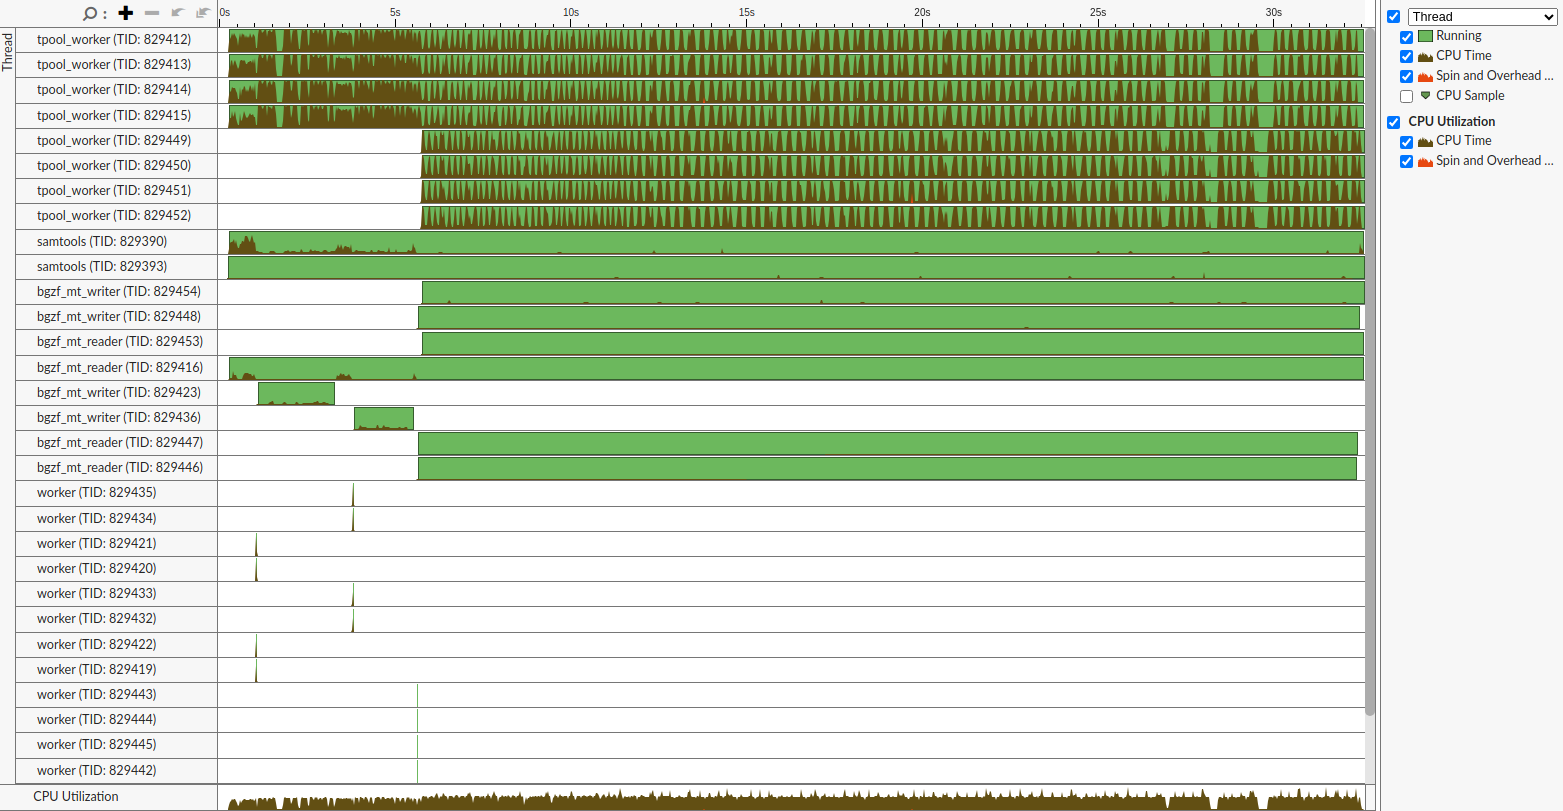
\includegraphics[width=1.5\linewidth]{figures/timelinePipe.png}}
% \caption{Screenshot of the VTune profiler on running \sort piped to SAMtools \texttt{view}. Both commands utilize 4 threads. However, the total of 8 CPUs the testing machine provides is never reached, as visualized under CPU Utilization. After 5.7 seconds, \sort starts merging the two temporary files it created before into the pipeline. The pipeline's buffer size is 1\,MB and the resulting file has a size of 230\,MB. In the merging and writing phase of \sort, 230 alternating spikes in CPU Time in the workers responsible for compression and decompression of \sort (first 4 rows) and SAMtools \texttt{view} can be found, indicating compression being a bottleneck of the piped operation.} \label{fig1}
% \end{figure}



\newpage

%
% ---- Bibliography ----
%
% BibTeX users should specify bibliography style 'splncs04'.
% References will then be sorted and formatted in the correct style.
%
\bibliographystyle{splncs04}
\bibliography{refs,references}

\end{document}
